\chapter{Cap\'{\i}tulo 4: Modelo de regresi\'{o}n ZOIP con efectos mixtos}\label{cap4}
%{\Huge \textbf{Modelo de regresi\'{o}n ZOIP con efectos mixtos\\}}

Los modelos de regresi\'{o}n mixtos han sido de mucho inter\'{e}s en la \'{u}ltima \'{e}poca, por su capacidad de estimar el efecto de una variable sobre el modelo, a trav\'{e}s de la estimaci\'{o}n de la varianza de la distribuci\'{o}n de la variable, estos fueron introducidos de una manera general por \cite{Laird1}. Es por esto que los modelos de regresi\'{o}n mixtos tambi\'{e}n han sido implementados cuando la variable respuesta es tomada por una variable aleatoria perteneciente a datos proporcionales, tal es el caso de \cite{Stasinopoulos2} en los modelos aditivos generalizados para localizaci\'{o}n, escala y forma (Gamlss) que implementan el modelo de regresi\'{o}n beta con intercepto aleatorio normal, as\'{\i} otros autores como \cite{Verkuilen1} y \cite{Bonat1} proponen modelos de regresi\'{o}n beta con efectos aleatorios normales, estimados a partir de m\'{a}xima verosimilitud marginal y metodolog\'{\i}as bayesianas. \cite{Figueroa1} extienden el modelo propuesto por \cite{Ferrari2} a un modelo con efectos fijos y aleatorios bajo la distribuci\'{o}n normal y bajo la distribuci\'{o}n t en estructuras de regresi\'{o}n tanto para el par\'{a}metro de la media, como del par\'{a}metro de precisi\'{o}n, la estimaci\'{o}n de los par\'{a}metros del modelo de regresi\'{o}n fue realizado bajo una perspectiva bayesiana, mediante implementaciones computacionales del muestreador de Gibbs. \cite{Usuga1} desarrollan el modelo de regresi\'{o}n beta mixto para datos proporcionales longitudinales, bajo intercepto y pendiente aleatoria normal y no normal, la estimaci\'{o}n de los par\'{a}metros es realizada v\'{\i}a m\'{a}xima verosimilitud y la cuadratura de Gauss-Hermite adaptativa. Otros autores como \cite{Song1} implementan un modelo de regresi\'{o}n mixto para una variable respuesta bajo la distribuci\'{o}n simplex, \cite{Bonat2} tambi\'{e}n realiza un an\'{a}lisis de verosimilitud del modelo beta mixto, donde la estimaci\'{o}n de los par\'{a}metros de regresi\'{o}n es realizada bajo algoritmos MCMC.\\

Como se pudo notar anteriormente, se ve que las metodolog\'{\i}as de estimaci\'{o}n de los pa\-r\'{a}\-me\-tros del modelo de regresi\'{o}n mixto no tienen una soluci\'{o}n cerrada anal\'{\i}ticamente y es un poco m\'{a}s complicada cuando se trata de una variable respuesta perteneciente a datos proporcionales, por lo que se utilizan ciertas aproximaciones o en la mayor\'{\i}a de los casos metodolog\'{\i}as y algoritmos bayesianos para la estimaci\'{o}n de los par\'{a}metros regresores. Una de las metodolog\'{\i}as utilizadas es la aproximaci\'{o}n de la funci\'{o}n de verosimilitud v\'{\i}a la cuadratura de Gauss-Hermite adaptativa, utilizada e implementada en los modelos de regresi\'{o}n beta mixtos por \cite{Usuga1} y es utilizada para la estimaci\'{o}n del modelo de regresi\'{o}n ZOIP mixto, dicha cuadratura fue implementada anteriormente por \cite{Fahrmeir1} sobre los modelos lineales generalizados. Diversos estudios para la estimaci\'{o}n de par\'{a}metros sobre modelos estad\'{\i}sticos han sido implementados mediante esta t\'{e}cnica, por ejemplo, el trabajo realizado por \cite{Liu1} y \cite{Smithson1} que estima los par\'{a}metros del modelo de regresi\'{o}n beta bajo la cuadratura de Gauss-Hermite. Por otra parte, se han realizado diversas modificaciones sobre la cuadratura de Gauss-Hermite original, tales como la cuadratura de Gauss-Hermite adaptativa y algunas mejoras sobre esta como la cuadratura de Gauss-Hermite adaptativa con \textit{pruning} \citep{Hernandez1}.\\

Los modelos de regresi\'{o}n mixtos que se han mencionado anteriormente sobre datos proporcionales, no se encuentran con presencia de datos en cero y/o uno, es decir inflados con ceros y/o unos, por lo que otros autores como \cite{Ospina2} presentaron una distribuci\'{o}n beta inflada con ceros o con unos, mediante una combinaci\'{o}n de una distribuci\'{o}n discreta y una distribuci\'{o}n continua dada por la distribuci\'{o}n beta con parametrizaci\'{o}n de \cite{Ferrari2} y la cual dio pie para que m\'{a}s adelante \cite{Ospina1} propusieran una clase general de modelos de regresi\'{o}n beta inflados en cero y uno. Recientemente \cite{Kosmidis1} han estudiado los modelos de regresi\'{o}n inflados para datos proporcionales, pero basados en una distribuci\'{o}n distinta a la propuesta por \cite{Ospina1}, sin embargo, cabe aclarar que los anteriores modelos son modelos de regresi\'{o}n para efectos fijos, es decir, no incluyen alg\'{u}n efecto aleatorio, por lo que otros autores como \cite{Galvis1} incluyen efectos aleatorios dentro de los modelos de regresi\'{o}n inflados con ceros y/o unos, basados en la distribuci\'{o}n propuesta por \cite{Ospina2}y otras distribuciones para datos proporcionales, como la distribuci\'{o}n simplex y beta-rectangular, la estimaci\'{o}n de los par\'{a}metros de regresi\'{o}n se realiz\'{o} mediante metodolog\'{\i}as bayesianas, MCMC.\\

Este cap\'{\i}tulo se encuentra organizado de la siguiente manera: primero se presenta el modelo de regresi\'{o}n ZOIP mixto basado en la distribuci\'{o}n ZOIP visto en el cap\'{\i}tulo \ref{cap2} y su debida estimaci\'{o}n, mediante m\'{a}xima verosimilitud, se muestra los diferentes tipos de cuadratura de Gauss-Hermite, para que posteriormente se muestre la aproximaci\'{o}n de la funci\'{o}n de verosimilitud v\'{\i}a la cuadratura de Gauss-Hermite adaptativa multidimensional, en la si\-gui\-en\-te secci\'{o}n se presenta la implementaci\'{o}n del modelo de regresi\'{o}n ZOIP mixto en el paquete \pkg{ZOIP} de \proglang{R} y por \'{u}ltimo se presenta unas aplicaciones a datos simulados y a datos reales.


%%%%%%%%%%%%%%%%%%%%%%%%%%%%%%%%%%%%%%%%%%%%%%%%%%%%%%%%%%%%%%%%%%%%%%%%%%%%%%%%%%%%%%%%%%%%%%%%%%%%%%%%%%%%%%%%%%%%%%%%%%%%%%%%%%%%%%%%%%%%%%%%%%%%%%%%%%%%%%%%%%

\section{Modelo de regresi\'{o}n ZOIP mixto}


Una escritura jer\'{a}rquica de dos niveles considerada para un modelo con variable respuesta dada por la distribuci\'{o}n para datos proporcionales inflados con ceros y/o unos (ZOIP), vista en la secci\'{o}n \ref{Sec_dist_zoip}. Denotando a $y_{ij}$ como la $j-$\'{e}sima medida del $i-$\'{e}simo grupo, adem\'{a}s si asumisos interceptos aleatorios $\gamma_{i1}$ y $\gamma_{i2}$, los cuales son independientes y cada uno sigue una distribuci\'{o}n normal con media cero y desviaci\'{o}n est\'{a}ndar $\lambda_1$ y $\lambda_2$, respectivamente. Asumimos tambi\'{e}n que los interceptos aleatorios $\gamma_{i1}$ y $\gamma_{i2}$ son independientes entre s\'{\i}. Una escritura matem\'{a}tica para el modelo es el siguiente:

\[
y_{ij}| \gamma_{i1},\gamma_{i2} \overset{\text{ind}}{\sim} ZOIP(\mu_{ij},\sigma_{ij},p_{0ij}, p_{1ij}),
\]
\[
\gamma_{i1} \overset{\text{i.i.d}}{\sim}  N(0,\lambda_1^2),
\]
\[
\gamma_{i2} \overset{\text{i.i.d}}{\sim}  N(0,\lambda_2^2),
\]
\\
Para $i=1,2,\ldots, N$ y $j=1,2,\ldots, n_i$ Los par\'{a}metros $\mu$, $\sigma$, $p_0$ y $p_1$ son modelados linealmente en funci\'{o}n de un conjunto de covariables respectivamente, por:


\[
h_1(\mu_{ij})=\mathbf{x}_{ij1}^{\top} \boldsymbol{\beta}_1+ \gamma_{i1},
\]
\[
h_2(\sigma_{ij})=\mathbf{x}_{ij2}^{\top} \boldsymbol{\beta}_2+ \gamma_{i2},
\]
\[
h_3(p_{0ij})=\mathbf{x}_{ij3}^{\top} \boldsymbol{\beta}_3,
\]
\[
h_4(p_{1ij})=\mathbf{x}_{ij4}^{\top} \boldsymbol{\beta}_4
\]


donde $\mathbf{x}_{ij1}$, $\mathbf{x}_{ij2}$, $\mathbf{x}_{ij3}$ y $\mathbf{x}_{ij4}$, son vectores de covariables conocidos de dimensi\'{o}n $k_1$, $k_2$, $k_3$ y $k_4$ respectivamente. $\boldsymbol{\beta}_1$, $\boldsymbol{\beta}_2$, $\boldsymbol{\beta}_3$ y $\boldsymbol{\beta}_4$ son vectores de par\'{a}metros desconocidos fijos asociados a las covariables y $\gamma_{i1}$, $\gamma_{i2}$ son los interceptos aleatorios asociados al $i-$\'{e}simo grupo. Adem\'{a}s las funciones $h_1(\cdot)$, $h_2(\cdot)$, $h_3(\cdot)$ y $h_4(\cdot)$ son funciones de enlace conocidas y apropiadas para mapear de los reales a los valores admisibles del par\'{a}metro, ademas son funciones estrictamente mon\'{o}tonas y doblemente diferenciables. Las posibles funciones para el par\'{a}metro $\mu$ y $\sigma$ son logit, probit, clog-log, o log dependiendo de la parametrizaci\'{o}n, para los par\'{a}metros de inflaci\'{o}n $p_0$ y $p_1$ son posibles funciones de enlace como logit, probit, clog-log.

\subsection{Inferencia estad\'{\i}stica}

Para la estimaci\'{o}n de los par\'{a}metros del modelo de regresi\'{o}n con intercepto aleatorio en la media y la varianza, para datos proporcionales inflados con ceros y/o unos, por medio de m\'{a}xima verosimilitud, es necesario hallar la funci\'{o}n de verosimilitud.

Considere $\boldsymbol{\theta}=(\boldsymbol{\beta_1}^{\top},\boldsymbol{\beta_2}^{\top},\boldsymbol{\beta_3}^{\top}, \boldsymbol{\beta_4}^{\top},\lambda_1,\lambda_2)^{\top}$ un vector de par\'{a}metros a ser estimado en el espacio:
\[
\Theta=\left\{\boldsymbol{\theta} \in \mathbb{R}^k | \boldsymbol{\beta_1} \in \mathbb{R}^{k_1}, \boldsymbol{\beta_2} \in \mathbb{R}^{k_2}, \boldsymbol{\beta_3} \in \mathbb{R}^{k_3}, \boldsymbol{\beta_4} \in \mathbb{R}^{k_4}, \lambda_1 \in \mathbb{R}^+, \lambda_2 \in \mathbb{R}^+  \right\}
\]

en el que $k=k_1+k_2+k_3+k_4+2$, tenemos que una distribuci\'{o}n marginal de $\mathbf{y}_i=(y_{1i},\ldots, y_{n_i}i)^{\top}$ es dada por:

\[
f(\mathbf{y}_i;\boldsymbol{\theta})=\int_{\mathbb{R}^2}\prod_{j=1}^{n_i}f(y_{ij}|\gamma_{i1},\gamma_{i2};\boldsymbol{\beta_1}, \boldsymbol{\beta_2}, \boldsymbol{\beta_3}, \boldsymbol{\beta_4})\cdot f(\gamma_{i1};\lambda_1) f(\gamma_{i2};\lambda_2) d\gamma_{i1}d\gamma_{i2},
\]

Entonces una funci\'{o}n de verosimilitud para las observaciones $\mathbf{y}=(y_1, \cdots, y_N)^{\top}$ es de la forma:

\[
L(\boldsymbol{\theta})=\prod_{i=1}^{N}f(\mathbf{y}_i;\boldsymbol{\theta})
\]
\[
=\prod_{i=1}^{N}\int_{\mathbb{R}^2}\prod_{j=1}^{n_i}f(y_{ij}|\gamma_{i1},\gamma_{i2};\boldsymbol{\beta_1}, \boldsymbol{\beta_2}, \boldsymbol{\beta_3}, \boldsymbol{\beta_4})\cdot f(\gamma_{i1};\lambda_1) f(\gamma_{i2};\lambda_2) d\gamma_{i1}d\gamma_{i2},
\]

\begin{equation}
\ell(\boldsymbol{\theta})=\sum_{i=1}^{N}log \left[\int_{\mathbb{R}^2}\prod_{j=1}^{n_i}f(y_{ij}|\gamma_{i1},\gamma_{i2};\boldsymbol{\beta_1}, \boldsymbol{\beta_2}, \boldsymbol{\beta_3}, \boldsymbol{\beta_4})\cdot f(\gamma_{i1};\lambda_1) f(\gamma_{i2};\lambda_2) d\gamma_{i1}d\gamma_{i2}\right],
 \label{func_ver_mix}
\end{equation}


donde $f(y_{ij}|\gamma_{i1},\gamma_{i2};\boldsymbol{\beta_1}, \boldsymbol{\beta_2}, \boldsymbol{\beta_3}, \boldsymbol{\beta_4})$ es la funci\'{o}n de densidad de probabilidad condicional de $y_{ij}$ que distribuye $ZOIP(\mu,\sigma,p_0,p_1)$. $\gamma_{i1}$, $\gamma_{i2}$ y $f(\gamma_{i1};\lambda_1)$ y $f(\gamma_{i2};\lambda_2)$ son funciones de densidades de probabilidad normales de $\gamma_{i1}$ y $\gamma_{i2}$, respectivamente. Para encontrar el m\'{a}ximo de la funci\'{o}n $\ell(\boldsymbol{\theta})$ no es posible mediante una manera cerrada anal\'{\i}ticamente, una dificultad adicional es la soluci\'{o}n de la integral para encontrar la maximizaci\'{o}n de la funci\'{o}n $\ell(\boldsymbol{\theta})$, por lo que es necesario utilizar t\'{e}cnicas computacionales para la soluci\'{o}n de esta, t\'{e}cnicas tales como aproximaciones de Laplace, algoritmos EM, integraci\'{o}n Monte Carlo o t\'{e}cnicas bayesianas. Para solucionar dicha funci\'{o}n de log-verosimilitud se utilizo el m\'{e}todo de integraci\'{o}n num\'{e}rica Gauss-Hermite adaptativa multidimensional con y sin \textit{pruning}, tal como se describe en la siguiente secci\'{o}n.


\subsection{Cuadratura de Gauss-Hermite}\label{sec:Cuadratura}

\subsubsection{Cuadratura de Gauss-Hermite unidimensional}

La cuadratura de Gauss-Hermite (GQ) es una herramienta \'{u}til para aproximar una integral de una funci\'{o}n $g(x)$ sobre $\Re$ con una suma ponderada, donde la variable $x$ es reemplazada por una cuadratura de $n$ puntos o nodos. Cada punto de la cuadratura es denotado por $p_i$, es evaluado en la funci\'{o}n y los resultados son ponderados por los pesos de la cuadratura asociados $w_i$.
\[
\int_\Re{g(x)dx}\approx\sum_{i=1}^{n}{g(p_i)exp(p_i^2)w_i.}
\]
\\
El conjunto de los $n$ puntos de la cuadratura $\textbf{P}=\left\{p_1,p_2,\ldots,p_n\right\}$ corresponde a las ra\'{\i}ces del polinomio de Hermite dado por:

\[
H_n{(x)}=(-1)^ne^{-x^2}\frac{d^n}{dx^n}e^{-x^2},
\]
\\
con pesos asociados $\textbf{W}=\left\{w_1,w_2,\ldots,w_n\right\}$ dados por

\[
w_i=\frac{2^{n-1}n!\sqrt{\pi}}{n^2{[H_{n-1}(x_i)]}^2}.
\]

\subsubsection{Cuadratura de Gauss-Hermite adaptativa}

\textbf{Unidimensional\\}
La cuadratura de Gauss-Hermite adaptativa (AGQ) es propuesta por \cite{Liu1}; \citep{Pinheiro1}, es b\'{a}sicamente una transformaci\'{o}n de los puntos asociados a la cuadratura, centrando y extendiendo alrededor del m\'{a}ximo valor de $\hat{x}$ de la funci\'{o}n $log(g(x))$. La transformaci\'{o}n de los puntos de la cuadratura $p_i$ definido como $p_i^*$, est\'{a} dado por \\
$p_i^*=\sqrt{2}\hat{\sigma}p_i+\hat{x}$ donde:

\[
\hat{\sigma}^2={\left[\left. -\frac{d^2}{dx^2}log(g(x))\right|_{x=\hat{x}}\right]^{-1}}.
\]
\\
As\'{\i}, la aproximaci\'{o}n de la integral de $g(x)$ sobre $\Re$ est\'{a} dado por:

\[
\int_\Re{g(x)dx}\approx\sqrt{2}\hat{\sigma}\sum_{i=1}^{n}{g(p_i^*)exp(p_i^2)w_i.}
\]

\textbf{Multidimensional\\}
Si extendemos la AGQ a una integral de dimensi\'{o}n q de la funci\'{o}n $g(x)$ sobre $\Re^q$, en este caso, con una cuadratura de $n$ puntos, $\textbf{Z}$ est\'{a} basado en el producto cartesiano de $\textbf{P}$, y los pesos de la cuadratura de $\textbf{A}$ est\'{a}n basados similarmente en el producto Kronecker, denotado por $\otimes$, los pesos originales $\textbf{W}$, son dados:

\[
\textbf{Z}=\underbrace{P \times \ldots \times P}_{q\ \text{veces}}=P^q,
\]

\[
\textbf{A}=\underbrace{W \otimes \ldots \otimes W}_{q\ \text{veces}}.
\]
\\
As\'{\i}, la expresi\'{o}n para la integral aproximada de $g(x)$ sobre $\Re^q$ est\'{a} dado por:

\[
\int_{\Re^q}{g(x)dx}\approx|\hat{Q}|^{1/2} 2^{q/2}\sum_{i=1}^{n^q}g(z_i^*)exp(z_i^{\top}z_i)a_i,
\]
\\
donde $z_i$ y $a_i$ corresponden a los elementos de $\textbf{Z}$ y $\textbf{A}$, respectivamente. Los nuevos puntos de la cuadratura $z_i^*$ estan centrados en el m\'{a}ximo de $\hat{x}$ del $log(g(x))$ y est\'{a} dado por \\
$z_i^*=\hat{x}+\sqrt{2}\hat{Q}^{1/2}z_i$, donde $\hat{Q}^{1/2}$ corresponde a la descomposici\'{o}n de Cholesky de la curvatura de la matriz $\hat{Q}$, que se encuentra dada por:

\[
\hat{Q}={\left[\left. -\frac{d^2}{dx^2}log(g(x))\right|_{x=\hat{x}}\right]^{-1}}.
\]

\subsubsection{Cuadratura de Gauss-Hermite adaptativa con \textit{pruning}}

Es claro que los resultados obtenidos por la AGQ son mejores que los de GQ, debido a que se encuentran centrados, sin embargo, la AGQ requiere un tiempo de optimizaci\'{o}n m\'{a}s elevado, debido a la transformaci\'{o}n de los puntos de cuadratura, pero no todos los puntos de la AGQ aportan de manera significativa un valor sobre la soluci\'{o}n de la integral, es por esto que \cite{Hernandez1} desarrolla un mejoramiento de la AGQ, donde elimina los puntos de la cuadratura que no son significativos sobre la soluci\'{o}n de la integral, de modo que no afectan de manera significativa los resultados finales de la integral, pero si afectan de manera positiva el tiempo de ejecuci\'{o}n, dicho mejoramiento es llamado cuadratura de Gauss-Hermite con \textit{pruning}.\\

La cuadratura de Gauss-Hermite adaptativa con \textit{pruning} consiste en eliminar puntos de la cuadratura, tales que el peso $a_i$ asociado al punto es menor que un valor de referencia $\theta$, que est\'{a} dado por:
\[
\theta=\frac{w_{[1]}w_{[\frac{n+1}{2}]}}{n^{q-1}}.
\]
\\
donde $w_{[1]}$ y $w_{[\frac{n+1}{2}]}$ corresponden respectivamente, a el valor m\'{\i}nimo y la mediana de los pesos originales \textbf{W}. (Ver m\'{a}s en \cite{Hernandez1}.)


\subsection{Aproximaci\'{o}n de la funci\'{o}n de verosimilitud v\'{\i}a cuadratura de Gauss-Hermite}

En la funci\'{o}n de verosimilitud definida en \eqref{func_ver_mix} se tiene que para cada i-esimo grupo se debe resolver la siguiente integral:

\begin{align*}
I_i &= \int_{\Re^2}{\prod_{j=1}^{n_i}f(y_{ij}|\gamma_{i1},\gamma_{i2};\boldsymbol{\beta_1}, \boldsymbol{\beta_2}, \boldsymbol{\beta_3}, \boldsymbol{\beta_4})\cdot f(\gamma_{i1};\lambda_1) f(\gamma_{i2};\lambda_2) d\gamma_{i1}d\gamma_{i2}}\\
&=\int_{\Re^2}{\prod_{j=1}^{n_i}f(y_{ij}|\gamma_{i1},\gamma_{i2};\boldsymbol{\beta_1}, \boldsymbol{\beta_2}, \boldsymbol{\beta_3}, \boldsymbol{\beta_4})\cdot \frac{exp({\gamma_{i1}^2}/{2\lambda_1^2})}{\lambda_1\sqrt{2\pi}} \cdot \frac{exp({\gamma_{i2}^2}/{2\lambda_2^2})}{\lambda_2\sqrt{2\pi}} d\gamma_{i1}d\gamma_{i2}}
\end{align*}

Si se realiza el siguiente cambio de variables

\begin{equation*}
\begin{aligned}
b_{i1}&=\frac{\gamma_{i1}}{\sqrt{2}\lambda_1}\\
\therefore b_{i1}^2&=\frac{\gamma_{i1}^2}{2\lambda_1^2}\\
\therefore \gamma_{i1}&=\sqrt{2}\lambda_1b_{i1}\\
\end{aligned}
\quad
\begin{aligned}
b_{i2}&=\frac{\gamma_{i2}}{\sqrt{2}\lambda_2}\\
b_{i2}^2&=\frac{\gamma_{i2}^2}{2\lambda_2^2}\\
\gamma_{i2}&=\sqrt{2}\lambda_2 b_{i2}
\end{aligned}
\end{equation*}

Por lo anterior se tiene que la integral $I_i$ se convierte en:

\begin{equation}
I_i=\int_{\Re^2}{\prod_{j=1}^{n_i}f(y_{ij}|\sqrt{2}\lambda_1b_{i1},\sqrt{2}\lambda_2 b_{i2};\boldsymbol{\beta_1}, \boldsymbol{\beta_2}, \boldsymbol{\beta_3}, \boldsymbol{\beta_4})\cdot \frac{exp(-b_{i1}^2) exp(-b_{i2}^2)}{\pi} db_{i1}db_{i2}}
\label{Int_vero_mix}
\end{equation}

La integral definida en \eqref{Int_vero_mix} tiene una forma factible para ser aproximada usando la cuadratura de Gauss-Hermite adaptativa multidimensional con o sin \textit{pruning}, vista en la secci\'{o}n \ref{sec:Cuadratura}, de este modo la integral $I_i$ es aproximada por:

\[
I_i=\sum_{k_1=1}^{Q_1}{\sum_{k_2=1}^{Q_2}{\prod_{j=1}^{n_i}f(y_{ij}|\sqrt{2}\lambda_1 z_{k_1},\sqrt{2}\lambda_2 z_{k_2};\boldsymbol{\beta_1}, \boldsymbol{\beta_2}, \boldsymbol{\beta_3}, \boldsymbol{\beta_4})\cdot \frac{w_{k_1}w_{k_2}}{\pi}}}
\]

donde $z_{k_1}$ y $z_{k_2}$ son los puntos de la cuadratura, $w_{k_1}$ y $w_{k_2}$ son los pesos asociados a los puntos de la cuadratura, por lo tanto la funci\'{o}n de verosimilitud aproximada es dada por:

\[
L(\boldsymbol{\theta})=\prod_{i=1}^{N}{\left[\sum_{k_1=1}^{Q_1}{\sum_{k_2=1}^{Q_2}{\prod_{j=1}^{n_i}f(y_{ij}|\sqrt{2}\lambda_1 z_{k_1},\sqrt{2}\lambda_2 z_{k_2};\boldsymbol{\beta_1}, \boldsymbol{\beta_2}, \boldsymbol{\beta_3}, \boldsymbol{\beta_4})\cdot \frac{w_{k_1}w_{k_2}}{\pi}}}\right]}
\]

y la funci\'{o}n de log verosimilitud esta dada por:

\begin{equation}
\ell(\boldsymbol{\theta})=\sum_{i=1}^{N}log{\left[\sum_{k_1=1}^{Q_1}{\sum_{k_2=1}^{Q_2}{\prod_{j=1}^{n_i}f(y_{ij}|\sqrt{2}\lambda_1 z_{k_1},\sqrt{2}\lambda_2 z_{k_2};\boldsymbol{\beta_1}, \boldsymbol{\beta_2}, \boldsymbol{\beta_3}, \boldsymbol{\beta_4})\cdot \frac{w_{k_1}w_{k_2}}{\pi}}}\right]}
\label{LOG_vero_mix}
\end{equation}

Al tener la funci\'{o}n de log verosimilitud definida en \eqref{LOG_vero_mix}, para hallar los estimadores m\'{a}ximos veros\'{\i}miles se debe utilizar herramientas computacionales, como algoritmos de optimizaci\'{o}n, tales como las funciones de \proglang{R}, \code{nlminb} o \code{optim}. La metodolog\'{\i}a de estimaci\'{o}n de los pa\-r\'{a}\-me\-tros del modelo de regresi\'{o}n ZOIP con intercepto aleatorio en la media y la varianza, utilizando m\'{a}xima verosimilitud v\'{\i}a cuadratura de Gauss-Hermite adaptativa multidimensional con o sin \textit{pruning}, se encuentra implementada en el paquete \pkg{ZOIP} de \proglang{R}, por medio de la funci\'{o}n \code{RMM.ZOIP}.

%%%%%%%%%%%%%%%%%%%%%%%%%%%%%%%%%%%%%%%%%%%%%%%%%%%%%%%%%%%%%%%%%%%%%%%%%%%%%%%%%%%%%%%%%%%%%%%%%%%%%%%%%%%%%%%%%%%%%%%%%%%%%%%%%%%%%%%%%%%%%%%%%%%%%%%%%%%%%%%%%%%%%%%%%%%%%%%%%%%%%%%
\section{Modelo de regresi\'{o}n ZOIP mixto en el paquete \pkg{ZOIP}}

En esta secci\'{o}n se mostrara como ajustar un modelo de regresi\'{o}n ZOIP con interceptos aleatorios en los par\'{a}metros de media y varianza, mediante el paquete \pkg{ZOIP} de \proglang{R}, utilizando el m\'{e}todo de m\'{a}xima verisimilitud y su aproximaci\'{o}n mediante la cuadratura de Gauss-Hermite adaptativa multidimensional con \textit{pruning} o sin \textit{pruning}.

\subsection{Funci\'{o}n RMM.ZOIP} 

La funci\'{o}n \code{RMM.ZOIP} estima los par\'{a}metros de un modelo regresi\'{o}n ZOIP con y sin covariables y con interceptos aleatorios en los par\'{a}metros de la media y la dispersi\'{o}n, dicha estimaci\'{o}n se realiza v\'{\i}a m\'{a}xima verosimilitud utilizando la cuadratura de Gauss-Hermite adaptativa multidimensional con o sin \textit{pruning}, adem\'{a}s se utilizara el optimizador \code{nlminb} o \code{optim} para la estimaci\'{o}n de los efectos fijos. La estructura de la funci\'{o}n \code{RMM.ZOIP} es la siguiente:

\begin{verbatim}
RMM.ZOIP(formula.mu, formula.sigma = ~1, formula.p0 = ~1, 
    formula.p1 = ~1, data, formula.random, link = c("identity", 
        "identity", "identity", "identity"), family = "R-S", 
    optimizer = "nlminb", n.points = 11, pruning = TRUE)
\end{verbatim}

Los argumentos de la funci\'{o}n \code{RMM.ZOIP} son:


\begin{itemize}[noitemsep, nolistsep]

\item \code{formula.mu}: Formula que define la funci\'{o}n de regresi\'{o}n de efectos fijos, para el par\'{a}metro $\mu$, un valor posible es \code{y $\sim$ x1 + x2}, es necesario definir la variable respuesta (y).
\item \code{formula.sigma}: Formula que define la funci\'{o}n de regresi\'{o}n de efectos fijos, para el par\'{a}metro $\sigma$, un valor posible es \code{$\sim$ x1}, por defecto \code{$\sim$ 1}.
\item \code{formula.p0}: Formula que define la funci\'{o}n de regresi\'{o}n de efectos fijos, para el par\'{a}metro $p_0$, un valor posible es \code{$\sim $x1}, por defecto \code{$\sim $1}.
\item \code{formula.p1}: Formula que define la funci\'{o}n de regresi\'{o}n de efectos fijos, para el par\'{a}metro $p_1$, un valor posible es \code{$\sim $x1}, por defecto \code{$\sim $1}.
\item \code{data}: Es el conjunto de datos en formato \code{data.frame} donde debe contener las nombres de las columnas tal cual como est\'{a}n en las f\'{o}rmulas.
\item \code{formula.random}: Formula que define el efecto mixto dentro del modelo, debe ser solo el intercepto aleatorio que se tendr\'{a} en cuenta en el par\'{a}metro de la media y la dispersi\'{o}n, la estructura admisible es la siguiente \code{formula.random = ~1 | G1}, donde \code{G1} es la variable que indica los grupos o sujetos en el modelo, siempre debe ser definido.
\item \code{family}: Elecci\'{o}n de la parametrizaci\'{o}n de la distribuci\'{o}n beta o distribuci\'{o}n deseada en la parte continua de la distribuci\'{o}n ZOIP, si toma el valor de \code{``R-S''} se utilizara la distribuci\'{o}n beta con parametrizaci\'{o}n \cite{Stasinopoulos2}, si toma el valor de \code{``F-C''} se utilizara la distribuci\'{o}n beta parametrizaci\'{o}n \cite{Ferrari2}, el valor de \code{``Original''} se utilizara la distribuci\'{o}n beta con parametrizaci\'{o}n original, \code{``Simplex''} utilizar\'{a} la distribuci\'{o}n simplex.
\item \code{link}: Es un vector con las funciones enlace adecuadas para cada par\'{a}metro a estimar de acuerdo a las opciones escogidas en los par\'{a}metros de familia y formula. Si el modelo de regresi\'{o}n no posee covariables se debe utilizar como funci\'{o}n enlace la opci\'{o}n \code{identity}, independientemente del valor escogido en familia, opciones posibles son \code{logit}, \code{log}. Por defecto \code{link=c(``identity'',``identity'',``identity'',``identity'')}.
\item \code{optimizer}: Elecci\'{o}n del optimizador, utilizado para encontrar la convergencia de la m\'{a}xima verosimilitud en los par\'{a}metros de efectos fijos, se puede elegir el valor de \code{``nlminb''} o \code{``optim''}, por defecto \code{``nlminb''}
\item \code{n.points}: N\'{u}mero de puntos a utilizar en la aproximaci\'{o}n de la funci\'{o}n de ve\-ro\-si\-mi\-li\-tud por medio de la cuadratura de Gauss-Hermite adaptativa multidimensional, por defecto es 11, se recomienda no dar un valor muy grande a este par\'{a}metro, por que afectara de manera significativamente los tiempos de convergencia del modelo.
\item \code{pruning}: Es un valor booleano que indica si se utiliza \textit{pruning} o no, para la cuadratura de Gauss-Hermite adaptativa multidimensional, por defecto es TRUE.

\end{itemize}

En el siguiente ejemplo se mostrar\'{a} el ajuste de un modelo de regresi\'{o}n ZOIP mixto, el cual proviene de datos simulados, se muestra el c\'{o}digo utilizado para dicha simulaci\'{o}n, como se utiliza la funci\'{o}n \code{RMM.ZOIP} para ajustar el modelo y mostrar la salida del modelo, explicando cada uno de sus componentes de la salida y la utilizaci\'{o}n de la funci\'{o}n \code{summary} sobre el objeto de salida de la funci\'{o}n \code{RMM.ZOIP}. Los datos simulados son provenientes de una distribuci\'{o}n ZOIP con parametrizaci\'{o}n \cite{Stasinopoulos2} con par\'{a}metros, como $\mu$ y $\sigma$ que depender\'{a}n de un intercepto aleatorio y una covariable discreta definida como cantidad de d\'{\i}as (2, 10, 20, 40), los par\'{a}metros de inflaci\'{o}n son fijados como $p_0=p_1=0.1$, el n\'{u}mero de grupos o sujetos ser\'{a} fijado a partir de $N$, como 21 grupos.

Se carga el paquete \pkg{ZOIP} y se definen los diferentes valores de los par\'{a}metros de la distribuci\'{o}n ZOIP, para ser simulada.
\begin{verbatim}
library(ZOIP)
N <- 21  # Numeros de grupos o sujetos

Times <- c(2, 10, 20, 40)  # cantidad de dias

subject <- rep(1:N, each = length(Times))
# numero de sujetos en la muestra repetidos tantas veces
# haya dias

Days <- rep(Times, times = N)
b0i <- rep(rnorm(n = N, sd = 1), each = length(Times))
b1i <- rep(rnorm(n = N, sd = 0.5), each = length(Times))

neta <- (1.6 + b0i) - 1.3 * log(Days)
neta2 <- (0.1 + b1i) - 0.8 * log(Days)

mu <- 1/(1 + exp(-neta))
sigma <- 1/(1 + exp(-neta2))

p0 <- 0.1
p1 <- 0.1
\end{verbatim}

Se verifica que no hayan valores de $\mu$ y $\sigma$ iguales a unos y se simula los valores de la variable respuesta.

\begin{verbatim}
mu[mu == 1] <- 0.999
mu[mu == 0] <- 0.001

sigma[sigma == 1] <- 0.999
sigma[sigma == 0] <- 0.001

family <- "R-S"

Y <- rZOIP(n = length(mu), mu = mu, sigma = sigma, p0 = p0, 
    p1 = p1, family = family)
base <- data.frame(Y, Days, subject)
\end{verbatim}

Se definen los argumentos de la funci\'{o}n \code{RMM.ZOIP}, tales como las regresiones a ser ajustadas a cada uno de los par\'{a}metros de la distribuci\'{o}n ZOIP.

\begin{verbatim}
formula.mu <- Y ~ log(Days)
formula.sigma <- ~log(Days)
formula.p0 <- ~1
formula.p1 <- ~1

formula.random <- ~1 | subject

link <- c("logit", "logit", "identity", "identity")

optimizer <- "nlminb"
n.points <- 11
pruning <- TRUE

mod <- RMM.ZOIP(formula.mu = formula.mu, formula.sigma = formula.sigma, 
    formula.p0 = formula.p0, formula.p1 = formula.p1, data = base, 
    formula.random = formula.random, link = link, family = family, 
    optimizer = optimizer, n.points = n.points, pruning = pruning)
mod
\end{verbatim}

Los resultados obtenidos se muestran a continuaci\'{o}n.

\begin{verbatim}
## Call:
## RMM.ZOIP(formula.mu = formula.mu, formula.sigma = formula.sigma, 
##     formula.p0 = formula.p0, formula.p1 = formula.p1, data = base, 
##     formula.random = formula.random, link = link, family = family, 
##     optimizer = optimizer, n.points = n.points, pruning = pruning)
## 
##  Results: 
## 
##  Estimated fixed coefficients for h(mu): 
## (Intercept)   log(Days) 
##    1.845423   -1.331609 
## 
##  Estimated fixed coefficients for h(sigma): 
## (Intercept)   log(Days) 
##   0.2795793  -0.5611416 
## 
##  Estimated fixed coefficients for h(p0): 
## (Intercept) 
##  0.08319893 
## 
##  Estimated fixed coefficients for h(p1): 
## (Intercept) 
##   0.1191148 
##  Estimated random coefficients for h(mu) and h(sigma) 
##                                      log(.)
## Random Intercept mu    0.7610678 -0.2730329
## Random Intercept sigma 0.5038028 -0.6855703
## 
##  message 
## [1] "relative convergence (4)"
## 
##  time 
## [1] 227.48
## 
##  iterations 
## [1] 39
## 
##  Log-likelihood 
## [1] 15.75655
\end{verbatim}

En el anterior resultado se obtienen varios aspectos importantes de la salida del modelo y leyendo de arriba hacia abajo, se tienen primero que todo los efectos fijos ajustados al modelo de regresi\'{o}n para el par\'{a}metro de la media $\mu$, luego los efectos fijos estimados para el modelo de regresi\'{o}n del par\'{a}metro de dispersi\'{o}n $\sigma$, luego los par\'{a}metros ajustados para la regresi\'{o}n sobre el par\'{a}metro de inflaci\'{o}n de ceros $p_0$, despu\'{e}s los efectos estimados de la regresi\'{o}n del par\'{a}metro de inflaci\'{o}n de unos $p_1$, seguido de la estimaci\'{o}n de los interceptos aleatorios para $\mu$ y para $\sigma$, en ella se muestra una matriz donde la primera columna son los valores de la desviaci\'{o}n est\'{a}ndar asociada a la distribuci\'{o}n normal, es decir, el valor asociado a $\lambda_1$ y $\lambda_2$, dichos valores generan el efecto aleatorio sobre los par\'{a}metros de la media y la dispersi\'{o}n en su intercepto, respectivamente, la segunda columna nos muestra el valor del logaritmo natural de $\lambda_1$ y $\lambda_2$, respectivamente; luego el siguiente resultado es el valor de la log verosimilitud del modelo ajustado, para ser utilizados como posibles comparaciones entre modelos, despu\'{e}s se muestra un mensaje de convergencia heredado del algoritmo de optimizaci\'{o}n \code{nlminb} o \code{optim}, luego el tiempo que demoro el ajuste del modelo en segundos y por \'{u}ltimo el n\'{u}mero de iteraciones necesarias para la convergencia de encontrar la m\'{a}xima verosimilitud.

\begin{verbatim}
summary(mod)
## ---------------------------------------------------------------
## Fixed effects for logit(mu) 
## ---------------------------------------------------------------
##             Estimate Std. Error  z value  Pr(>|z|)    
## (Intercept)  1.84542    0.32408   5.6944 1.238e-08 ***
## log(Days)   -1.33161    0.10306 -12.9202 < 2.2e-16 ***
## ---
## Signif. codes:  0 *** 0.001 ** 0.01 * 0.05 . 0.1   1
## ---------------------------------------------------------------
## Fixed effects for logit(sigma) 
## ---------------------------------------------------------------
##             Estimate Std. Error z value  Pr(>|z|)    
## (Intercept)  0.27958    0.40333  0.6932    0.4882    
## log(Days)   -0.56114    0.12949 -4.3335 1.468e-05 ***
## ---
## Signif. codes:  0 *** 0.001 ** 0.01 * 0.05 . 0.1   1
\end{verbatim}
\begin{verbatim}
## ---------------------------------------------------------------
## Fixed effects for identity(p0) 
## ---------------------------------------------------------------
##             Estimate Std. Error z value Pr(>|z|)   
## (Intercept) 0.083199   0.030112   2.763 0.005727 **
## ---
## Signif. codes:  0 *** 0.001 ** 0.01 * 0.05 . 0.1   1
## ---------------------------------------------------------------
## Fixed effects for identity(p1) 
## ---------------------------------------------------------------
##             Estimate Std. Error z value  Pr(>|z|)    
## (Intercept) 0.119115   0.035352  3.3694 0.0007532 ***
## ---
## Signif. codes:  0 *** 0.001 ** 0.01 * 0.05 . 0.1   1
## ---------------------------------------------------------------
## ---------------------------------------------------------------
## Random effects for mu and sigma 
## ---------------------------------------------------------------
##                        Estimate Std. Error z value  Pr(>|z|)    
## Random Intercept mu     0.76107    0.23334  3.2616 0.0011077 ** 
## Random Intercept sigma  0.50380    0.14046  3.5867 0.0003349 ***
## ---
## Signif. codes:  0 *** 0.001 ** 0.01 * 0.05 . 0.1   1
## ---------------------------------------------------------------
## ---------------------------------------------------------------
\end{verbatim}

En el anterior resultado del paquete \pkg{ZOIP} se aplic\'{o} la funci\'{o}n de m\'{e}todo S3 \code{summary} al objeto que guardo la salida del modelo de regresi\'{o}n ZOIP mixto, esta funci\'{o}n dar\'{a} resultados m\'{a}s detallados de la estimaci\'{o}n de los par\'{a}metros, tendr\'{a} como resultado para cada par\'{a}metro de regresi\'{o}n del modelo ZOIP mixto, el valor estimado, el error est\'{a}ndar asociado, el valor Z de la distribuci\'{o}n normal y su respectivo valor p; esto ayudar\'{a} al usuario del paquete \pkg{ZOIP} a concluir con m\'{a}s argumentos el ajuste de sus par\'{a}metros y covariables dentro del modelo de regresi\'{o}n ZOIP mixto ajustado.
 
%%%%%%%%%%%%%%%%%%%%%%%%%%%%%%%%%%%%%%%%%%%%%%%%%%%%%%%%%%%%%%%%%%%%%%%%%%%%%%%%%%%%%%%%%%%%%%%%%%%%%%%%%%%%%%%%%%%%%%%%%%%%%%%%%%%%%%%%%%%%%%%%%%%%%%%%%%%%%%%%%%
\section{Aplicaci\'{o}n}

En esta secci\'{o}n se muestran diferentes resultados sobre el ajuste de un modelo de regresi\'{o}n ZOIP con intercepto aleatorio en el par\'{a}metro de la media y la varianza, por medio del paquete \pkg{ZOIP}, primero se realiz\'{o} el ajuste de un modelo de regresi\'{o}n ZOIP mixto sobre datos reales, aplicado al porcentaje de utilizaci\'{o}n de la tarjeta de cr\'{e}dito (tdc), valorado por el efecto de la ciudad donde vive la persona que le pertenece la tdc, segundo se realiz\'{o} un estudio de simulaci\'{o}n del modelo de regresi\'{o}n ZOIP mixto, basado en la aplicaci\'{o}n a datos reales, este estudio nos permite analizar la convergencia de la estimaci\'{o}n de los pa\-r\'{a}\-me\-tros asociados a los efectos fijos y aleatorios del modelo de regresi\'{o}n mixto, adem\'{a}s poder analizar y determinar cu\'{a}l es la mejor alternativa para estimar los modelos de regresi\'{o}n ZOIP mixto, sobre las diferentes opciones de utilizar la cuadratura de Gauss-Hermite adaptativa multidimensional.

\subsection{Datos reales}

En una entidad financiera es de importancia estudiar los efectos de ciertas variables sobre el porcentaje de utilizaci\'{o}n de las tarjetas de cr\'{e}dito de la entidad, porque esto dar\'{a} respuestas a activaci\'{o}n de campa\~{n}as publicitarias y estudios de mercadeo para incentivar la utilizaci\'{o}n de las tdc, de acuerdo a la situaci\'{o}n o caracter\'{\i}sticas de la persona due\~{n}a de la tdc, es por esto que en esta secci\'{o}n se analiz\'{o} el efecto que tiene la variable \textsl{Total mora} y la \textsl{ciudad}, sobre el porcentaje de utilizaci\'{o}n de la tdc. La variable \textsl{Total mora} nos indica el n\'{u}mero de meses que la tarjeta ha entrado en mora en toda la vida de la tdc; la \textsl{ciudad} nos indicara donde vive el cliente a quien pertenece de la tdc. Estas dos variables son importantes para la entidad financiera, porque indicar\'{a} o estimar\'{a} el porcentaje de utilizaci\'{o}n de una tdc para cuando un cliente ha llegado a estar en mora varios meses y vive en cierta ciudad, por lo que indicar\'{a} a la entidad financiera, como actuar sobre ciertas personas de inter\'{e}s. Para poder cuantificar dicho efecto se plante\'{o} un modelo de regresi\'{o}n ZOIP-beta con intercepto aleatorio en el par\'{a}metro de la media y la varianza, dado por la variable \textsl{ciudad} y un efecto fijo en la media y la varianza dado por la variable \textsl{Total mora}, el modelo es planteado bajo la distribuci\'{o}n ZOIP-beta con parametrizaci\'{o}n de \cite{Stasinopoulos2}. El n\'{u}mero de datos con que se cuenta es un total de 15 tarjetas de cr\'{e}dito por cada ciudad, el n\'{u}mero de ciudades tomadas en cuenta son 10 (Bogot\'{a}, Medell\'{\i}n, Cali, Barranquilla, Bucaramanga, Cartagena, C\'{u}cuta, Ibagu\'{e}, Envigado y Neiva), para as\'{\i} obtener una base total de 150 tdc. el modelo planteado se muestra a continuaci\'{o}n:\\

Si $y_{ij}| \gamma_{i1},\gamma_{i2} \overset{\text{ind}}{\sim} ZOIP(\mu_{ij},\sigma_{ij},p_0, p_1),$

\begin{equation}
\begin{split}
&h_1(\mu_{ij})=\beta_0+\gamma_{1i}+\beta_1 x_{1ij},\\
&h_2(\sigma_{ij})=\beta_0+\gamma_{2i}+\beta_1 x_{1ij},\\
&h_3(p_{0ij})=\beta_0,\\
&h_4(p_{1ij}) =\beta_0,
\end{split}
\label{A_eq_reg_mix}
\end{equation}

donde $y_{ij}$ es porcentaje de utilizaci\'{o}n de la j-esima tdc perteneciente a la i-esima ciudad, $i=1,2,\ldots, 10$, es decir, $N=10$ asociada a las 10 ciudades; $j=1,2,\ldots, 15$, es decir, $n_i=15$ asociada al n\'{u}mero de tdc por cada ciudad, en este caso todas las ciudades tienen el mismo n\'{u}mero de observaciones, es decir, se cuenta con una muestra balanceada; $x_{1ij}$: es el valor del n\'{u}mero de meses en mora de la j-esima tdc asociada a la i-esima ciudad; $\gamma_{1i}$ y $\gamma_{2i}$ son los interceptos aleatorios para los par\'{a}metros de la media y la varianza, respectivamente, asociados a la i-esima ciudad y provenientes de la distribuci\'{o}n normal con media cero y desviaci\'{o}n est\'{a}ndar $\lambda_1$ para el par\'{a}metro regresor $\gamma_{1i}$ y $\lambda_2$ para el par\'{a}metro regresor $\gamma_{2i}$. Las funciones enlaces asociadas a cada regresi\'{o}n se tomaran como una funci\'{o}n $logit$, esto debido a que el modelo de regresi\'{o}n ZOIP-beta mixto se plante\'{o} bajo la parametrizaci\'{o}n de \cite{Stasinopoulos2} y este deber\'{a} utilizar dicha funci\'{o}n enlace, tal cual como se explic\'{o} en el cap\'{\i}tulo anterior.\\


\begin{table}[!hbt]
{\scriptsize
\begin{center}
\begin{tabular}{|c|c|c|c|c|}\hline
& \multicolumn{4}{|c|}{Par\'{a}metros regresores} \\ \hline
Par\'{a}metro & $\hat{\beta}_0$ (Error est\'{a}ndar)&  $\hat{\beta}_1$ (Error est\'{a}ndar) & $\hat{\lambda}_1$ (Error est\'{a}ndar)& $\hat{\lambda}_2$ (Error est\'{a}ndar) \\ \hline
$\mu$ & -1.13 (0.24)	&0.33	(0.13)&0.51 (0.30)& \\ \hline
$\sigma$ & 0.33	(0.20)&0.14	(0.09)&	&0.40 (0.31) \\ \hline
$p_0$ & 0.23 (0.03)& & & \\ \hline
$p_1$ & 0.07 (0.02)& & & \\ \hline
\end{tabular}
\caption{Estimaci\'{o}n de los efectos fijos y aleatorios del modelo de regresi\'{o}n ZOIP mixto para el porcentaje utilizaci\'{o}n de una tdc.}
\label{T_Apli_mix}
\end{center}
}
\end{table}

En la tabla \ref{T_Apli_mix} se muestra la estimaci\'{o}n de los efectos fijos y aleatorios del modelo de regresi\'{o}n ZOIP-beta mixto, estimado v\'{\i}a m\'{a}xima verosimilitud y mediante la aproximaci\'{o}n de la cuadratura de Gauss-Hermite adaptativa multidimensional, utilizando 11 puntos de cuadratura con \textit{pruning}. En esta tabla se evidencia como al tener un numero de meses en mora m\'{a}s alto se aumenta el porcentaje medio y la varianza de utilizaci\'{o}n de las tdc, adem\'{a}s se observa que $\hat{\lambda}_1=0.51$ dando as\'{\i} que $\gamma_{1i} \sim N(0, 0.51)$, lo que nos permite ver el efecto del cambio de ciudad sobre el porcentaje medio de utilizaci\'{o}n de las tdc, el valor $\hat{\lambda}_2$ es de $0.4$, evidenciando que $\gamma_{2i} \sim N(0, 0.4)$, lo que nos indicar\'{a} cuantificar el efecto del cambio de ciudad sobre la variabilidad del porcentaje de utilizaci\'{o}n de las tdc, por otra parte se evidencia que alrededor de un 20\% de las tdc no se utilizan para nada y que un 7\% tienen utilizado la totalidad de su cupo de la tarjeta de cr\'{e}dito. Por \'{u}ltimo el modelo fue ajustado mediante la funci\'{o}n \code{RMM.ZOIP} del paquete \pkg{ZOIP}, tardando un total de 83.5 segundos, un tiempo relativamente prudente para el ajuste un modelo complejo, como lo es el modelo de regresi\'{o}n ZOIP-beta mixto.\\

El modelo propuesto en \eqref{A_eq_reg_mix} se puede reescribir con los par\'{a}metros estimados como:
\[
y_{ij}| \gamma_{i1},\gamma_{i2} \overset{\text{ind}}{\sim} ZOIP(\mu_{ij},\sigma_{ij},p_0, p_1),
\]
\begin{equation}
\begin{split}
&h_1(\mu_{ij})=-1.13+\gamma_{1i}+0.33 x_{1ij},\\
&h_2(\sigma_{ij})=0.33+\gamma_{2i}+0.14 x_{1ij},\\
&h_3(p_{0ij})=0.23,\\
&h_4(p_{1ij}) =0.07,
\end{split}
\label{A_eq_reg_mix2}
\end{equation}

donde $\gamma_{1i} \sim N(0, 0.51)$ y $\gamma_{2i} \sim N(0, 0.4)$.

\subsection{Datos simulados}

En esta secci\'{o}n se muestra la realizaci\'{o}n de un estudio de simulaci\'{o}n para verificar la convergencia de los par\'{a}metros regresores sobre los valores reales, adem\'{a}s se puede concluir a partir de este estudio, cual es la mejor metodolog\'{\i}a posible para la estimaci\'{o}n de los par\'{a}metros del modelo de regresi\'{o}n ZOIP mixto. Para dicho estudio se tom\'{o} en cuenta el modelo final estimado en la aplicaci\'{o}n a datos reales de la secci\'{o}n anterior, as\'{\i} como se describi\'{o} en el modelo estimado en \eqref{A_eq_reg_mix2}. Para poder encontrar la mejor metodolog\'{\i}a de estimaci\'{o}n del modelo de regresi\'{o}n ZOIP mixto se plantean 18 escenarios de simulaci\'{o}n y se realizaron 1000 r\'{e}plicas de cada escenario; los escenarios son resultantes de todas las combinaciones entre, variar el n\'{u}mero de puntos de la cuadratura de Gauss-Hermite ($Q=3 , Q=10, Q=20$), variar el tama\~{n}o de muestra de cada grupo o ciudad ($n_i=5, n_i=20, n_i=50$) y tener en cuenta si la cuadratura de Gauss-Hermite adaptativa multidimensional se realizar\'{a} con o sin \textit{pruning}.\\

\begin{figure}
	\begin{center}
		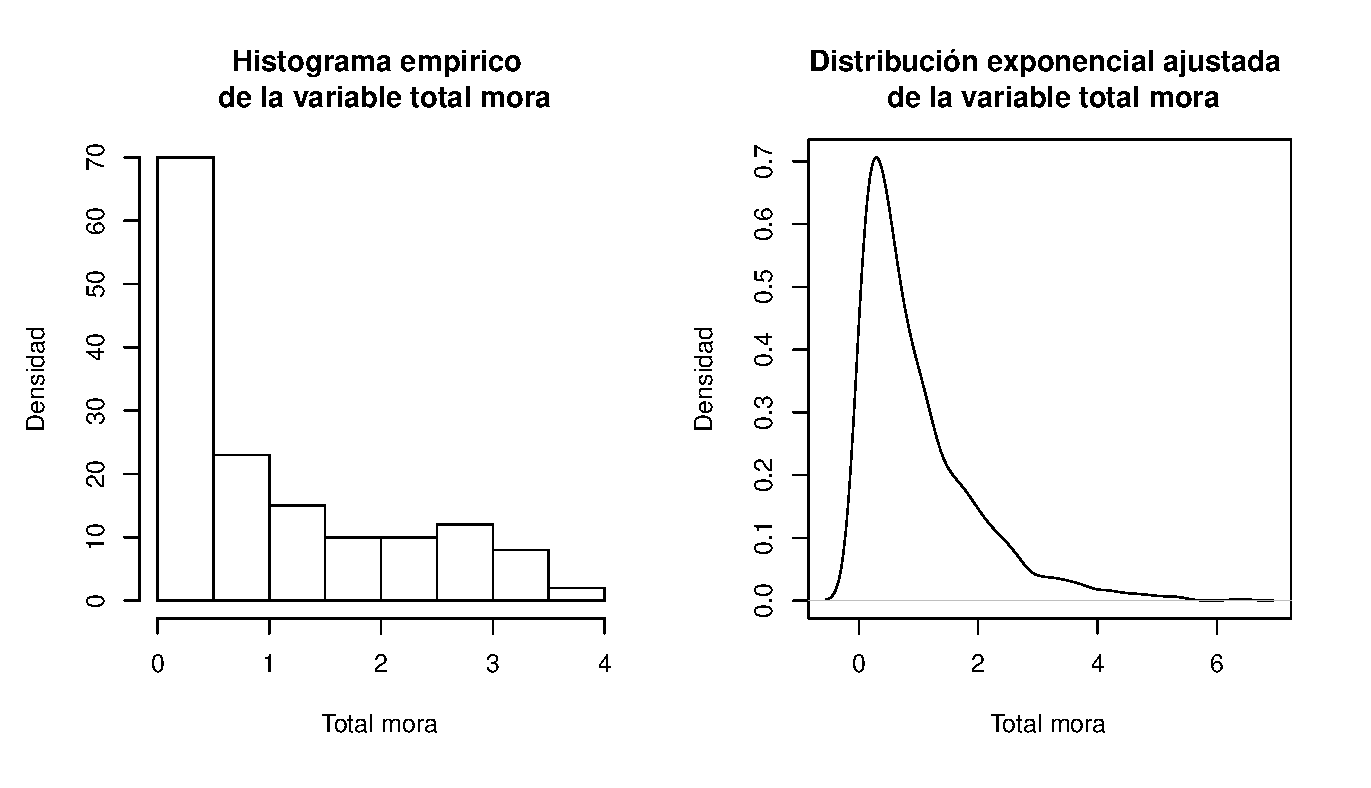
\includegraphics[scale=0.6]{Ajuste_expo_mix.eps}	
		\caption{Ajuste de la distribuci\'{o}n exponencial a la variable \textsl{Total mora}}
		\label{Ajuste_expo_mix}
	\end{center}
\end{figure}

Para poder variar el tama\~{n}o de muestra de cada ciudad es necesario encontrar la distribuci\'{o}n que genera la covariable \textsl{Total mora}. En la figura \ref{Ajuste_expo_mix} se muestra como la distribuci\'{o}n exponencial con par\'{a}metro $\lambda=1.075$ describe de forma adecuada el comportamiento de la variable \textsl{Total mora} descrita a partir de los datos reales obtenidos en la secci\'{o}n anterior.\\

Al tener la distribuci\'{o}n que genera los datos de la variable \textsl{Total mora}, permitir\'{a} obtener cualquier n\'{u}mero de observaciones de dicha variable, en particular el n\'{u}mero de muestras necesarias para los escenarios de simulaci\'{o}n propuestos, anteriormente. A continuaci\'{o}n se muestra los resultados de la simulaci\'{o}n del modelo de regresi\'{o}n ZOIP-beta mixto bajo la parametrizaci\'{o}n de \cite{Stasinopoulos2}, realizada bajo la funci\'{o}n \code{RMM.ZOIP} del paquete \pkg{ZOIP} de \proglang{R}.\\

\begin{table}[!hbt]
{\scriptsize
\begin{center}
\begin{tabular}{|c|c|c|c|c|c|c|c|}\hline
& & \multicolumn{3}{|c|}{Con \textit{pruning}} & \multicolumn{3}{|c|}{Sin \textit{pruning}} \\ \hline
Par\'{a}metro & $\beta$'s & $n_i=5$ & $n_i=20$ & $n_i=50$ & $n_i=5$ & $n_i=20$ & $n_i=50$ \\ \hline \hline
\multirow{3}{*}{$\mu$} & $\hat{\beta}_0$ & -1.137	&-1.110	&-1.076	&-1.128	&-1.120	&-1.080 \\ 
& $\hat{\beta}_1$ & 0.321	&0.327	&0.326	&0.331	&0.330	&0.327 \\
& $\hat{\lambda}_1$ & 0.879	&0.576	&0.507	&0.882	&0.568	&0.498 \\ \hline
\multirow{3}{*}{$\sigma$} & $\hat{\beta}_0$ & 0.445	&0.380	&0.336	&0.452	&0.377	&0.345 \\ 
& $\hat{\beta}_1$ & 0.072	&0.118	&0.132	&0.066	&0.121	&0.133\\
& $\hat{\lambda}_2$ & 0.728	&0.450	&0.396	&0.727	&0.456	&0.398\\ \hline
$p_0$& $\hat{\beta}_0$ &0.220	&0.230	&0.230	&0.220	&0.230	&0.230 \\ \hline
$p_1$& $\hat{\beta}_0$ &0.060	&0.070	&0.070	&0.060	&0.070	&0.072 \\ \hline
Tiempo(Seg)& &115.72	&130.85	&140.58	&61.69	&163.36	&218.68 \\ \hline
Nro Iteraciones& &22	&30	&34	&22	&30	&34 \\ \hline
\end{tabular}
\caption{Estimaci\'{o}n de los par\'{a}metros de regresi\'{o}n y los interceptos aleatorios de un modelo de regresi\'{o}n simulado ZOIP mixto, visto a partir del tama\~{n}o de muestra y si se utiliza \textit{pruning} o no.}
\label{T_Sim_mix_ni}
\end{center}
}
\end{table}

En la tabla \ref{T_Sim_mix_ni} se muestra los valores estimados de cada uno de los par\'{a}metros de las regresiones ajustadas con respecto al tama\~{n}o de muestra $n_i$ y si se utiliz\'{o} \textit{pruning} o no, los valores estimados de cada par\'{a}metro regresor y desviaci\'{o}n est\'{a}ndar de las distribuciones normales asociadas a los interceptos aleatorios, fueron hallados, a partir de la mediana de los valores estimados de las r\'{e}plicas de los escenarios de simulaci\'{o}n que cumplen con cada combinaci\'{o}n entre los diferentes tama\~{n}os de muestra y si fue con \textit{pruning} o no. En dicha tabla se nota como los valores de $\lambda_1$ y $\lambda_2$ asociados a los interceptos aleatorios van convergiendo a su valor real a trav\'{e}s que el tama\~{n}o de muestra va aumentando sin importar si se hizo con o sin \textit{pruning}, adem\'{a}s se nota como la estimaci\'{o}n de la pendiente va convergiendo a trav\'{e}s que le tama\~{n}o de muestra va creciendo, este par\'{a}metro da un valor muy plausible desde tama\~{n}os de muestra peque\~{n}os, sin importar si se hizo con o sin \textit{pruning}, este \'{u}ltimo fen\'{o}meno se evidencia tambi\'{e}n con los par\'{a}metros de inflaci\'{o}n en los que se tiene un valor muy cercano al real desde los tama\~{n}os de muestra peque\~{n}os. En cuesti\'{o}n del tiempo de ejecuci\'{o}n se ve como es reducido en aproximadamente un 50\%, cuando se utiliza la metodolog\'{\i}a de la cuadratura de Gauss-Hermite adaptativa con \textit{pruning}, con respecto a no utilizar \textit{pruning}. Sobre el n\'{u}mero de iteraciones se observa como al aumentar el tama\~{n}o de la muestra se requiere una cantidad de iteraciones m\'{a}s elevada.\\

\begin{table}[!hbt]
{\scriptsize
\begin{center}
\begin{tabular}{|c|c|c|c|c|c|c|c|}\hline
& & \multicolumn{3}{|c|}{Con \textit{pruning}} & \multicolumn{3}{|c|}{Sin \textit{pruning}} \\ \hline
Par\'{a}metro & $\beta$'s & $Q=3$ & $Q=10$ & $Q=20$ & $Q=3$ & $Q=10$ & $Q=20$ \\ \hline \hline
\multirow{3}{*}{$\mu$} & $\hat{\beta}_0$ & -1.122	& -1.069	& -1.120	& -1.117	& -1.076	& -1.129 \\ 
& $\hat{\beta}_1$ & 0.323	&0.322	&0.333	&0.334	&0.322	&0.329 \\
& $\hat{\lambda}_1$ & 0.632	&0.626	&0.634	&0.629	&0.616	&0.623 \\ \hline
\multirow{3}{*}{$\sigma$} & $\hat{\beta}_0$ & 0.400	&0.365	&0.366	&0.382	&0.379	&0.373 \\ 
& $\hat{\beta}_1$ & 0.117	&0.119	&0.120	&0.123	&0.117	&0.121 \\
& $\hat{\lambda}_2$ & 0.490	&0.487	&0.491	&0.501	&0.482	&0.486 \\ \hline
$p_0$& $\hat{\beta}_0$ &0.228	&0.228	&0.226	&0.226	&0.226	&0.226 \\ \hline
$p_1$& $\hat{\beta}_0$ &0.068	&0.070	&0.070	&0.070	&0.068	&0.070 \\ \hline
Tiempo(Seg)& &75.295	&128.28	&271.825	&74.295	&162.35	&367.545 \\ \hline
Nro Iteraciones& &30	&29	&29	&29	&29	&29 \\ \hline
\end{tabular}
\caption{Estimaci\'{o}n de los par\'{a}metros de regresi\'{o}n y los interceptos aleatorios de un modelo de regresi\'{o}n simulado ZOIP mixto, visto a partir del n\'{u}mero de puntos de la cuadratura y si se utiliza \textit{pruning} o no.}
\label{T_Sim_mix_ncua}
\end{center}
}
\end{table}

En la tabla \ref{T_Sim_mix_ncua} se muestran los valores estimados de cada uno de los par\'{a}metros de las regresiones ajustadas con respecto al n\'{u}mero de puntos utilizados en la cuadratura de Gauss-Hermite adaptativa $Q$ y si se utiliz\'{o} \textit{pruning} o no, los valores estimados de cada par\'{a}metro regresor y desviaci\'{o}n est\'{a}ndar de las distribuciones normales asociadas a los interceptos aleatorios fueron hallados, a partir de la mediana de los valores estimados de las r\'{e}plicas de los escenarios de simulaci\'{o}n que cumplen con cada combinaci\'{o}n entre los diferentes n\'{u}meros de puntos de cuadratura y si fue con \textit{pruning} o no. En dicha tabla se observa como en general cuando se utiliza una mayor cantidad de puntos de cuadratura se evidencia una peque\~{n}a mejora en la convergencia de los valores reales de los efectos fijos y aleatorios. Con respecto a la utilizaci\'{o}n de \textit{pruning} o no, se observa como las estimaciones de par\'{a}metros no tienen una diferencia significativa en la utilizaci\'{o}n de \textit{pruning} o no, por lo que es mejor utilizar la cuadratura de Gauss-Hermite adaptativa con \textit{pruning} por que al parecer se obtienen resultados similares, pero con una reducci\'{o}n significativa del tiempo de estimaci\'{o}n de los par\'{a}metros. El n\'{u}mero de iteraciones utilizadas para la estimaci\'{o}n de los par\'{a}metros no se ve influenciado por la cantidad de puntos utilizados en la cuadratura o si se utiliza \textit{pruning} o no.\\

\begin{figure}
	\begin{center}
		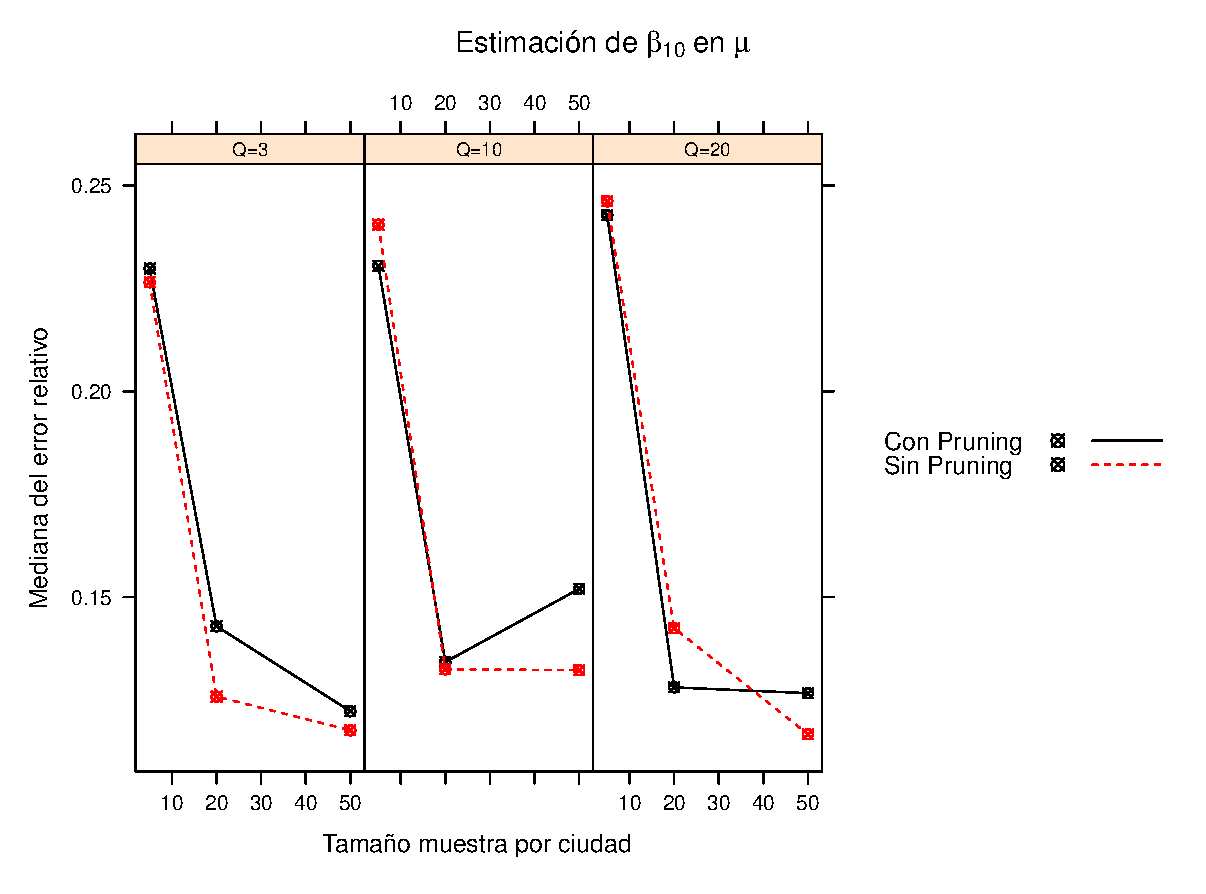
\includegraphics[scale=0.6]{MAPE_beta0_mu.eps}	
		\caption{Mediana del error relativo de la estimaci\'{o}n del par\'{a}metro $\beta0$ asociado a la media, variando el tama\~{n}o de muestra, el n\'{u}mero de puntos de la cuadratura y si utiliza \textit{pruning} o no.}
		\label{MAPE_bo_mu}
	\end{center}
\end{figure}

La mediana del error relativo de un par\'{a}metro estimado es calculado a partir de hallar el error relativo de las 1000 r\'{e}plicas de cada escenario de simulaci\'{o}n para cada par\'{a}metro estimado y calcularle la mediana a los mil valores calculados, el error relativo se puede definir como $|(\theta-\hat{\theta})/\theta|$, donde $\theta$ representa cualquier par\'{a}metro estimado en el modelo de regresi\'{o}n ZOIP mixto. \\

En la figura \ref{MAPE_bo_mu} se muestra la mediana del error relativo de variar el tama\~{n}o de muesta $n_i$, el n\'{u}mero de puntos de la cuadratura $Q$ y si se utiliza \textit{pruning} o no, sobre el intercepto fijo ($\hat{\beta}_0$) asociado a $\mu$, en dicha figura se muestra como el aumentar el tama\~{n}o de muestra en cada ciudad se obtiene una reducci\'{o}n de la mediana del error relativo de $\hat{\beta}_0$, sin embargo, al aumentar el n\'{u}mero de puntos de la cuadratura se obtienen errores muy parecidos en todos los tama\~{n}os de muestra, por lo que se podr\'{\i}a decir que el aumento del n\'{u}mero de puntos de cuadratura no mejora la estimaci\'{o}n del intercepto fijo sobre la media, por otra parte se obtienen errores relativos parecidos cuando se utiliza \textit{pruning} que cuando no, sin embargo, se puede rescatar que hay puntos como cuando el tama\~{n}o de muestra es 50 y $Q=10$ el error relativo de con \textit{pruning} es m\'{a}s grande del que no utiliza \textit{pruning}.\\

\begin{figure}
	\begin{center}
		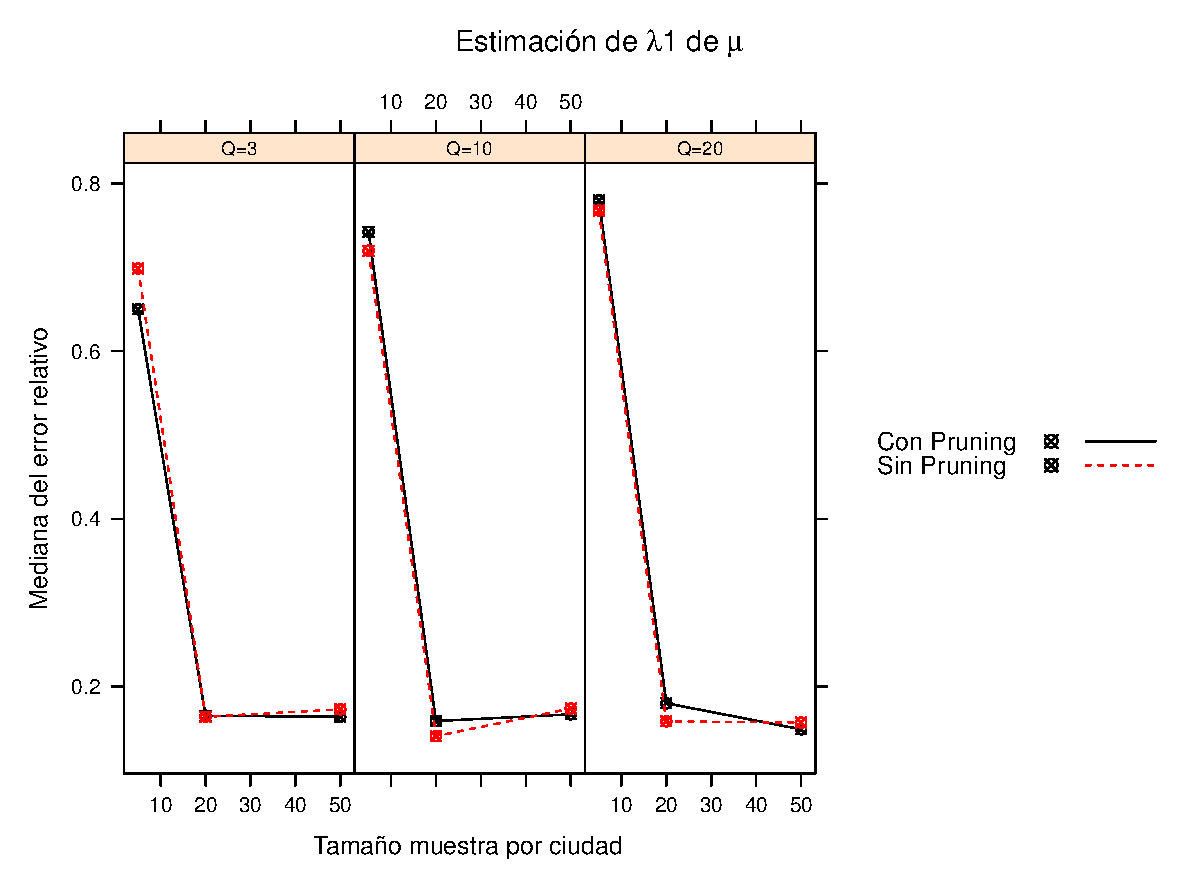
\includegraphics[scale=0.6]{MAPE_lambda1_mu.eps}	
		\caption{Mediana del error relativo de la estimaci\'{o}n del par\'{a}metro $\lambda_1$ desviaci\'{o}n est\'{a}ndar del intercepto aleatorio asociado a la media, variando el tama\~{n}o de muestra, el n\'{u}mero de puntos de la cuadratura y si utiliza \textit{pruning} o no.}
		\label{MAPE_lambda1_mu}
	\end{center}
\end{figure}

En la figura \ref{MAPE_lambda1_mu} se muestra la mediana del error relativo de variar el tama\~{n}o de muestra $n_i$, el n\'{u}mero de puntos de la cuadratura $Q$ y si se utiliza \textit{pruning} o no, sobre el valor de la desviaci\'{o}n est\'{a}ndar de la distribuci\'{o}n normal que genera el intercepto aleatorio ($\hat{\gamma}_{1i}$) del parametro de $\mu$, en dicha figura se muestra como el tama\~{n}o de muestra al ser aumentado obtiene una reducci\'{o}n significativa sobre la mediana del error relativo, adem\'{a}s al aumentar el n\'{u}mero de puntos de la cuadratura se obtienen errores menores cuando se aumentan el n\'{u}mero de puntos de la cuadratura, dicha mejora es de alrededor de un 2\% cuando el tama\~{n}o de muestra es m\'{a}s grande y $Q=20$, esto para cuando se utiliza \textit{pruning} y cuando no, por lo que se podr\'{\i}a decir que el aumento del n\'{u}mero de puntos de cuadratura mejora la estimaci\'{o}n del intercepto aleatorio sobre la media cuando el tama\~{n}o de muestra es relativamente grande, por otra parte se obtienen errores relativamente parecidos cuando se utiliza \textit{pruning} que cuando no.\\


\begin{figure}
	\begin{center}
		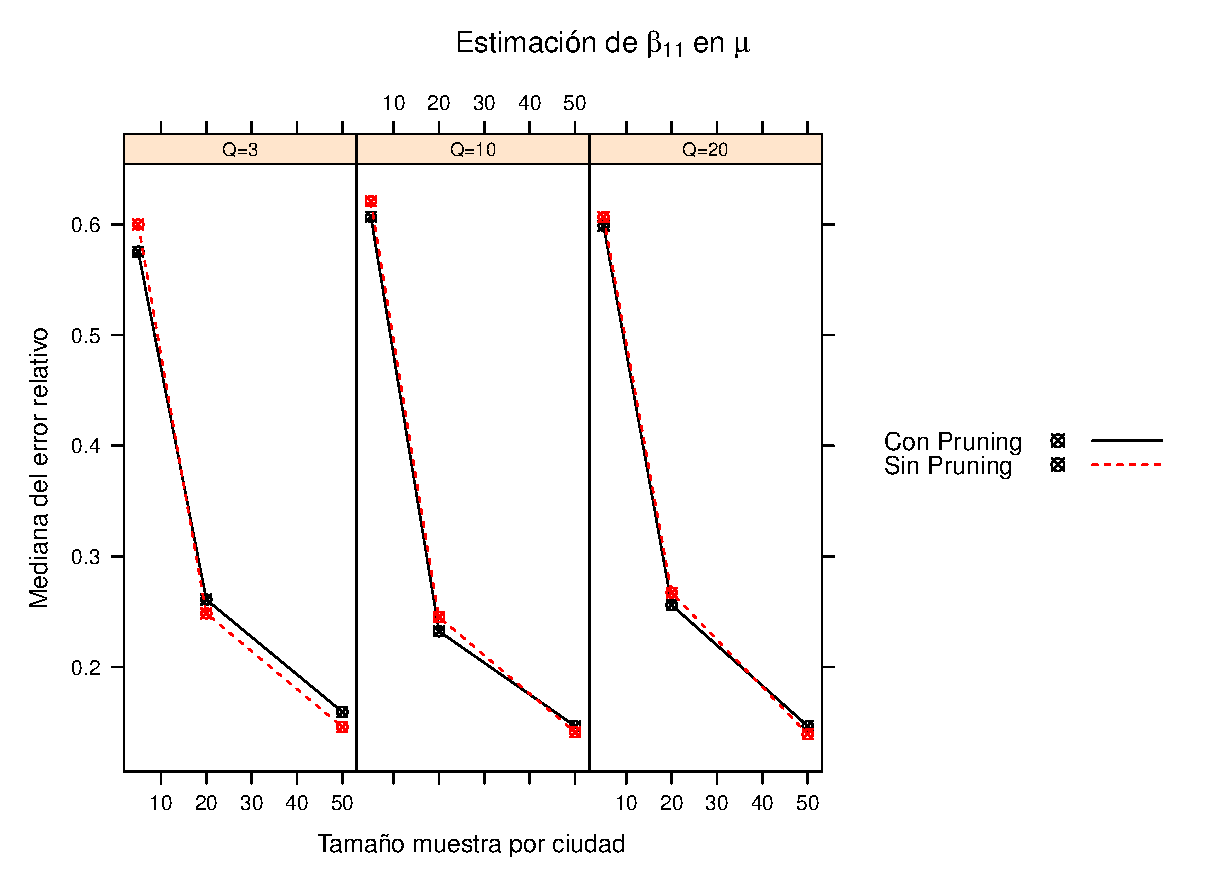
\includegraphics[scale=0.6]{MAPE_beta1_mu.eps}	
		\caption{Mediana del error relativo de la estimaci\'{o}n del par\'{a}metro $\beta1$ asociado a la media, variando el tama\~{n}o de muestra, el n\'{u}mero de puntos de la cuadratura y si utiliza \textit{pruning} o no.}
		\label{MAPE_beta1_mu}
	\end{center}
\end{figure}

En la figura \ref{MAPE_beta1_mu} se muestra la mediana del error relativo de variar el tama\~{n}o de muestra $n_i$, el n\'{u}mero de puntos de la cuadratura $Q$ y si se utiliza \textit{pruning} o no, sobre el valor del efecto fijo de la variable \textsl{Total mora} sobre la media, en dicha figura se muestra como el tama\~{n}o de muestra al ser aumentado obtiene una reducci\'{o}n de la mediana del error relativo, adem\'{a}s al aumentar el n\'{u}mero de puntos de la cuadratura se obtienen errores un poco menores, pero no significativo, cuando se aumentan el n\'{u}mero de puntos de la cuadratura, lo que nos permite observar que el aumento del n\'{u}mero de puntos de la cuadratura, no afecta demasiado en la estimaci\'{o}n de este efecto fijo, esto sin importar si se utiliza \textit{pruning} o no, por otra parte se obtienen errores muy parecidos cuando se utiliza \textit{pruning} y cuando no, esto no parece afectar la estimaci\'{o}n del par\'{a}metro.\\

\begin{figure}
	\begin{center}
		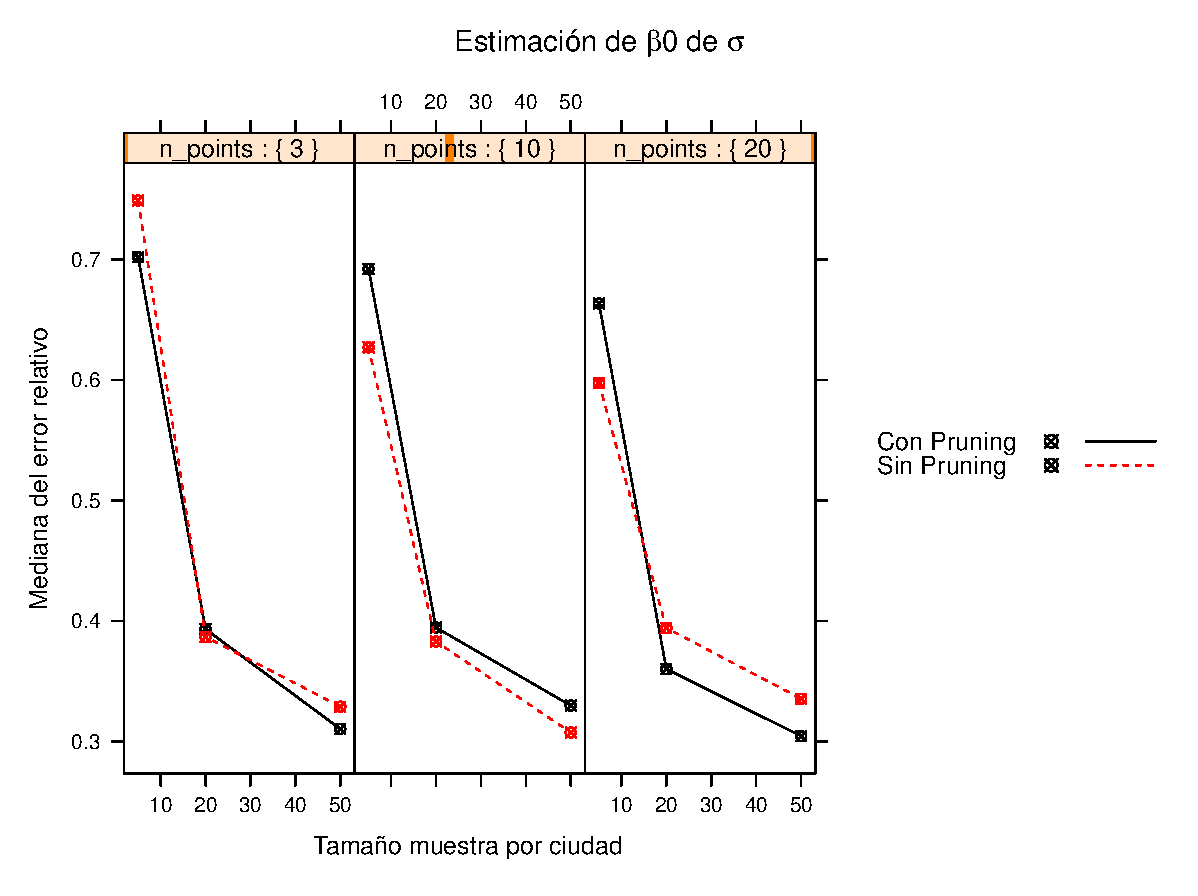
\includegraphics[scale=0.6]{MAPE_beta0_sigma.eps}	
		\caption{Mediana del error relativo de la estimaci\'{o}n del par\'{a}metro $\beta0$ asociado a la dispersi\'{o}n, variando el tama\~{n}o de muestra, el n\'{u}mero de puntos de la cuadratura y si utiliza \textit{pruning} o no.}
		\label{MAPE_beta0_sigma}
	\end{center}
\end{figure}

En la figura \ref{MAPE_beta0_sigma} se muestra la mediana del error relativo de variar el tama\~{n}o de muestra $n_i$, el n\'{u}mero de puntos de la cuadratura $Q$ y si se utiliza \textit{pruning} o no, sobre el intercepto fijo ($\hat{\beta}_0$) del par\'{a}metro de $\sigma$, en dicha figura se muestra como cuando se aumenta el tama\~{n}o de muestra en cada ciudad se obtiene una reducci\'{o}n de la mediana del error relativo, por otra parte al aumentar el n\'{u}mero de puntos de la cuadratura se obtienen errores muy parecidos en todos los tama\~{n}os de muestra, sin embargo, cuando $Q=20$ y se realiza sin \textit{pruning} se nota una reducci\'{o}n en el error, Ahora si observamos las medianas de los errores relativos son relativamente parecidos cuando se utiliza \textit{pruning} que cuando no, sin embargo, se puede rescatar que hay puntos como cuando el tama\~{n}o de muestra es 20 o 50 y el $Q=20$ el error relativo, de la metodolog\'{\i}a sin utilizar \textit{pruning} se ve reducido la mediana del error relativo, mejorando as\'{\i} la estimaci\'{o}n del par\'{a}metro.\\

\begin{figure}
	\begin{center}
		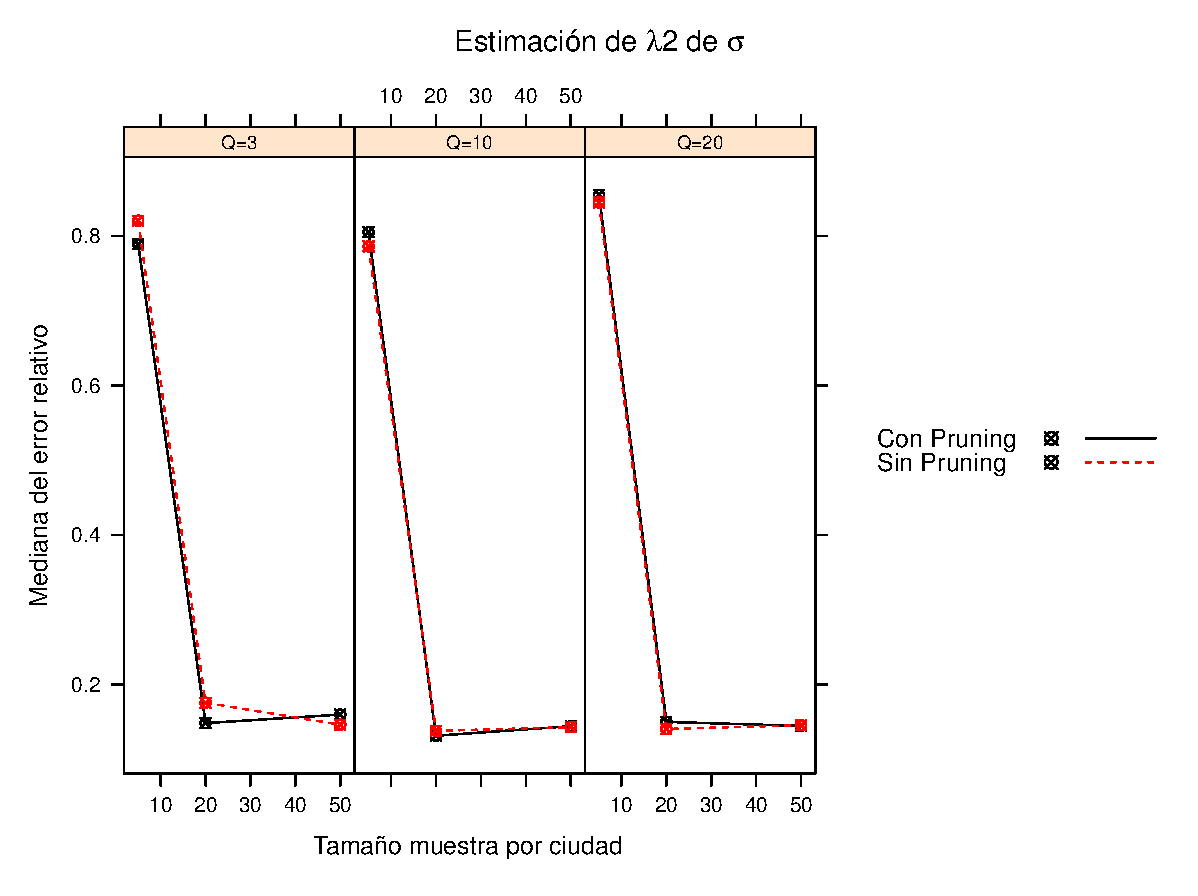
\includegraphics[scale=0.6]{MAPE_lambda2_sigma.eps}	
		\caption{Mediana del error relativo de la estimaci\'{o}n del par\'{a}metro $\lambda_2$ desviaci\'{o}n est\'{a}ndar del intercepto aleatorio asociado a la dispersi\'{o}n, variando el tama\~{n}o de muestra, el n\'{u}mero de puntos de la cuadratura y si utiliza \textit{pruning} o no.}
		\label{MAPE_lambda2_sigma}
	\end{center}
\end{figure}

En la figura \ref{MAPE_lambda2_sigma} se muestra la mediana del error relativo de variar, el tama\~{n}o de muestra $n_i$, el n\'{u}mero de puntos de la cuadratura $Q$ y si se utiliza \textit{pruning} o no, sobre el valor de la desviaci\'{o}n est\'{a}ndar de la distribuci\'{o}n normal que genera el intercepto aleatorio ($\hat{\gamma}_2$) del par\'{a}metro de $\sigma$, en dicha figura se muestra como el tama\~{n}o de muestra al ser aumentado obtiene una reducci\'{o}n de la mediana del error relativo de forma significativa, adem\'{a}s al aumentar el n\'{u}mero de puntos de la cuadratura se obtienen errores un poco menores, la mejora se nota a partir de $Q\geq10$, dicha mejora es de alrededor un 2\% cuando los tama\~{n}os de muestra de cada grupo es mayor que 10, no se nota una diferencia cuando se utiliza \textit{pruning} o cuando no, por lo que se podr\'{\i}a decir que el aumento del n\'{u}mero de puntos de cuadratura mejora la estimaci\'{o}n del intercepto aleatorio sobre la dispersi\'{o}n cuando el tama\~{n}o de muestra es relativamente grande, por otra parte se obtienen errores relativamente parecidos cuando se utiliza \textit{pruning} que cuando no, por lo que los valores de las estimaciones no se ven afectadas por la metodolog\'{\i}a \textit{pruning}.\\

\begin{figure}
	\begin{center}
		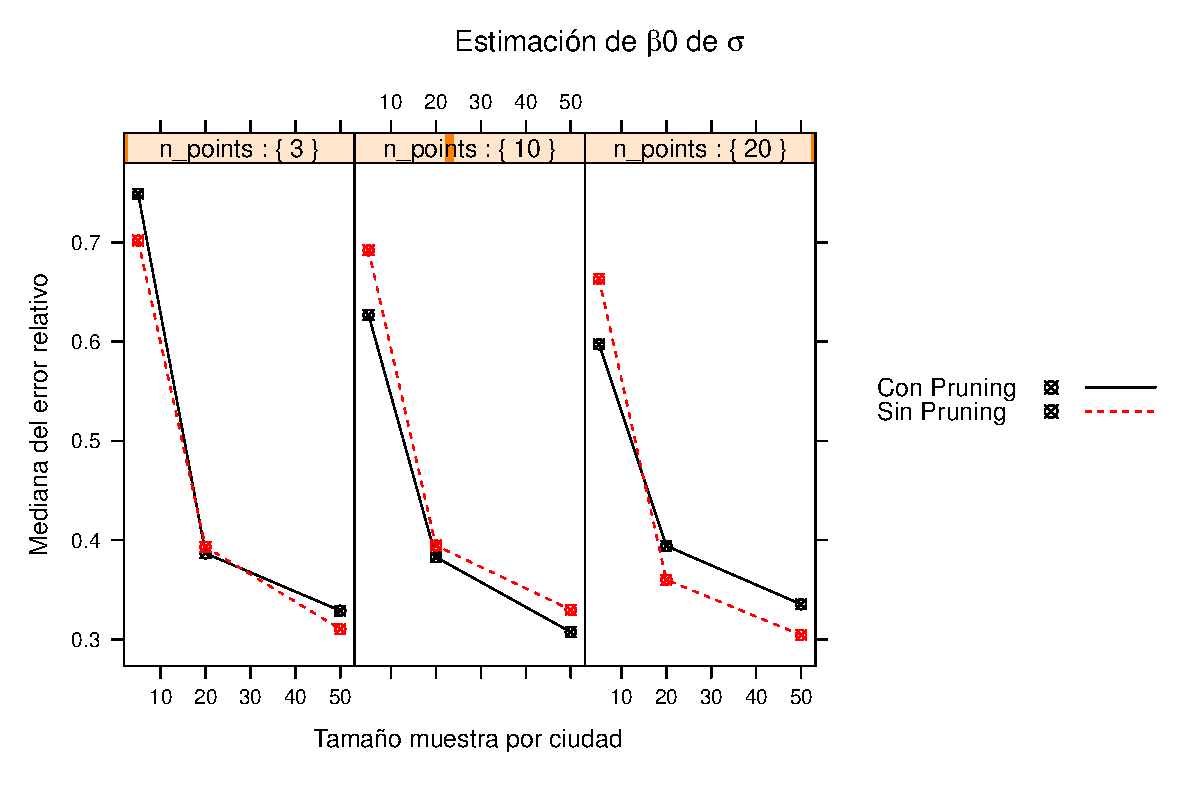
\includegraphics[scale=0.6]{MAPE_beta1_sigma.eps}	
		\caption{Mediana del error relativo de la estimaci\'{o}n del par\'{a}metro $\beta1$ asociado a la dispersi\'{o}n, variando el tama\~{n}o de muestra, el n\'{u}mero de puntos de la cuadratura y si utiliza \textit{pruning} o no.}
		\label{MAPE_beta1_sigma}
	\end{center}
\end{figure}

En la figura \ref{MAPE_beta1_sigma} se muestra la mediana del error relativo de variar, el tama\~{n}o de muestra $n_i$, el n\'{u}mero de puntos de la cuadratura $Q$ y si se utiliza \textit{pruning} o no, sobre el valor del efecto fijo de la variable \textsl{Total mora} sobre la dispersi\'{o}n, en dicha figura se muestra como el tama\~{n}o de muestra al ser aumentado obtiene una reducci\'{o}n de la median del error relativo, adem\'{a}s al aumentar el n\'{u}mero de puntos de la cuadratura no se obtiene una mejora significativa de la mediana del error relativo, Otro aspecto que es importante resaltar es que las estimaciones no se ven afectadas por el hecho de utilizar la metodolog\'{\i}a \textit{pruning} o no.\\

\begin{figure}
	\begin{center}
		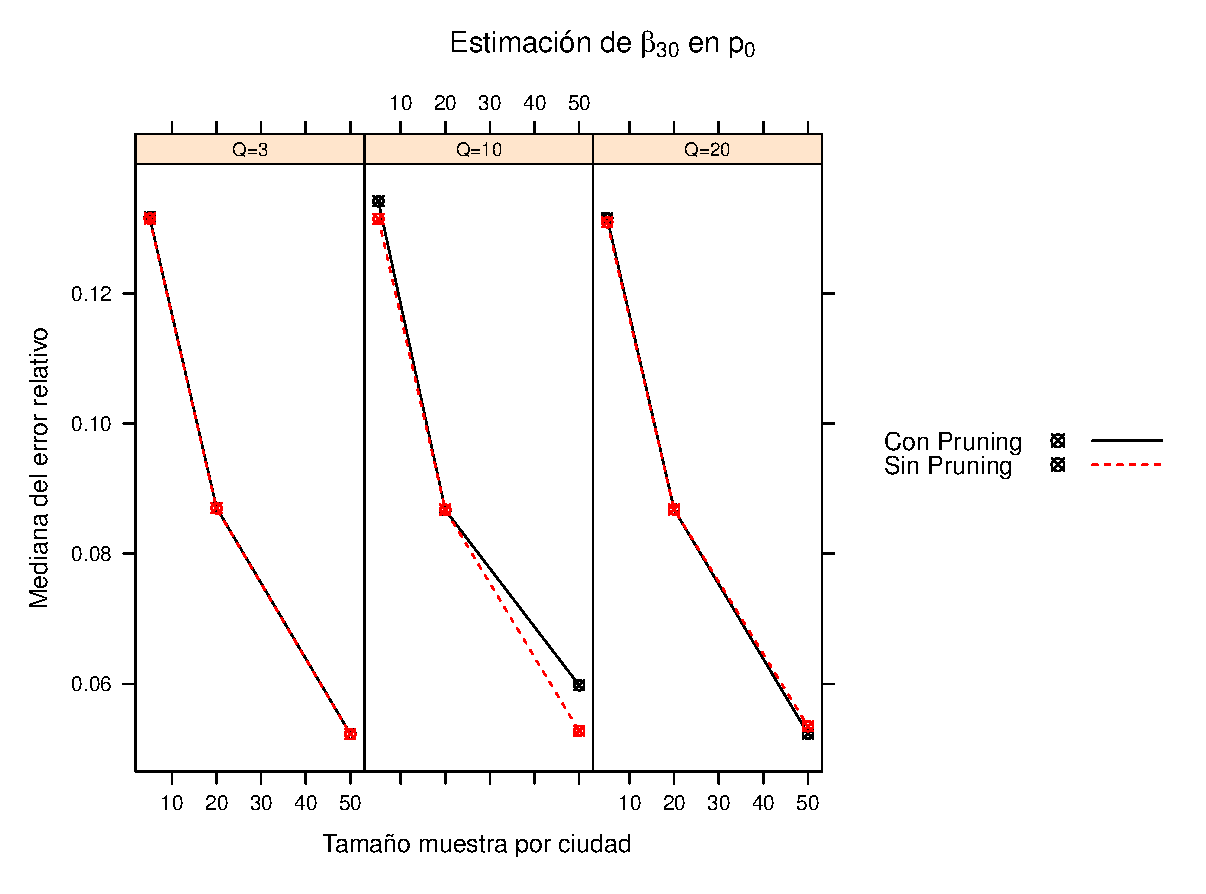
\includegraphics[scale=0.6]{MAPE_beta0_p0.eps}	
		\caption{Mediana del error relativo de la estimaci\'{o}n del par\'{a}metro $\beta0$ asociado al par\'{a}metro de inflaci\'{o}n de ceros, variando el tama\~{n}o de muestra, el n\'{u}mero de puntos de la cuadratura y si utiliza \textit{pruning} o no.}
		\label{MAPE_beta0_p0}
	\end{center}
\end{figure}

En la figura \ref{MAPE_beta0_p0} se muestra la mediana del error relativo de variar, el tama\~{n}o de muestra $n_i$, el n\'{u}mero de puntos de la cuadratura $Q$ y si se utiliza \textit{pruning} o no sobre el valor de la estimaci\'{o}n del porcentaje de ceros dentro del modelo de regresi\'{o}n ZOIP mixto, es estimado muy bien desde valores de tama\~{n}o de muestra peque\~{n}os, con una mediana del error relativo de alrededor del 13\%, sin embargo, se nota como a medida que el tama\~{n}o de muestra aumenta dicho error decrece r\'{a}pidamente; no se nota una diferencia al variar el n\'{u}mero de puntos de la cuadratura ni sobre la utilizaci\'{o}n de la metodolog\'{\i}a \textit{pruning}.\\

\begin{figure}
	\begin{center}
		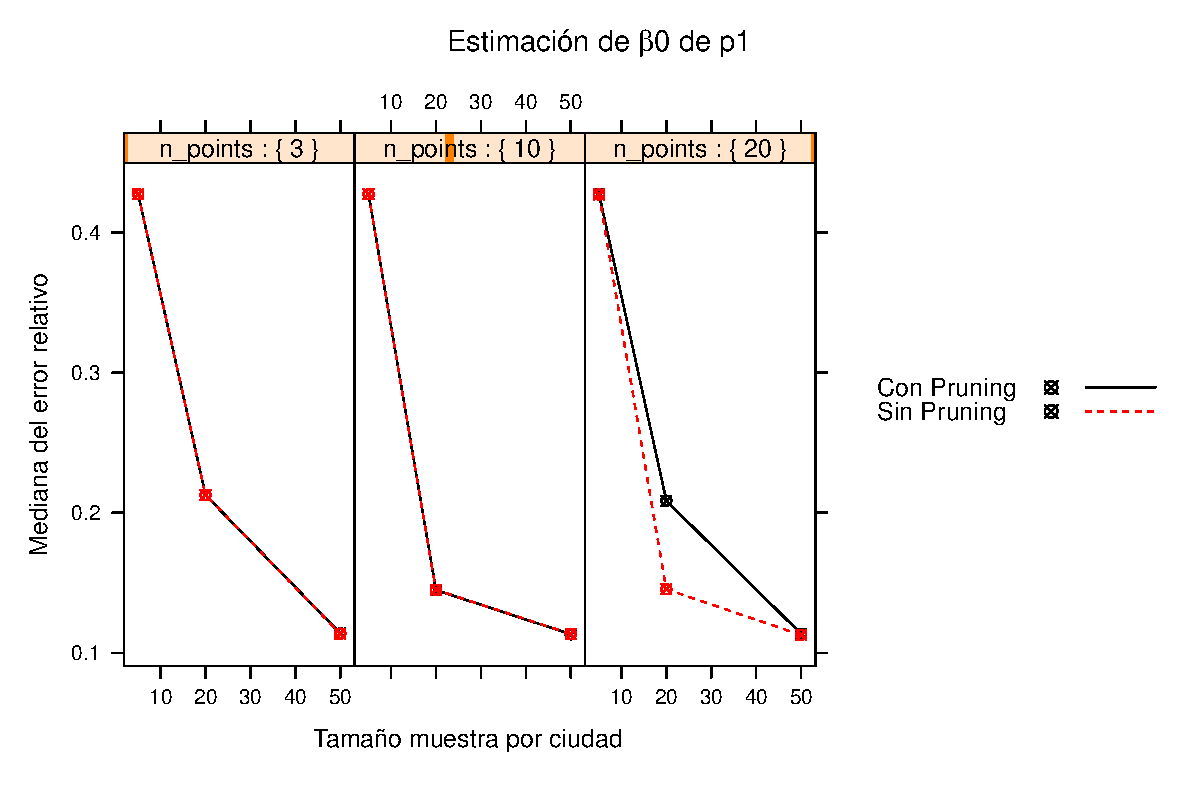
\includegraphics[scale=0.6]{MAPE_beta0_p1.eps}	
		\caption{Mediana del error relativo de la estimaci\'{o}n del par\'{a}metro $\beta0$ asociado al par\'{a}metro de inflaci\'{o}n de unos, variando el tama\~{n}o de muestra, el n\'{u}mero de puntos de la cuadratura y si utiliza \textit{pruning} o no.}
		\label{MAPE_beta0_p1}
	\end{center}
\end{figure}

En la figura \ref{MAPE_beta0_p1} se muestra la mediana del error relativo de variar, el tama\~{n}o de muestra $n_i$, el n\'{u}mero de puntos de la cuadratura $Q$ y si se utiliza \textit{pruning} o no, sobre el valor de la estimaci\'{o}n del porcentaje de unos dentro del modelo de regresi\'{o}n ZOIP mixto, la estimaci\'{o}n de este par\'{a}metro se ve afectado por el tama\~{n}o de muestra elegido dentro de cada grupo, ya que se nota como al aumentar el tama\~{n}o de muestra la mediana del error relativo decrece r\'{a}pidamente entre el tama\~{n}o de muestra $n_i=5$ y $n_i=20$ y decrece medianamente r\'{a}pido y entre los valores de $n_i$ 20 y 50. Adem\'{a}s se puede observar como no hay una diferencia entre la estimaci\'{o}n del par\'{a}metro variando del n\'{u}mero de puntos de la cuadratura ni tampoco sobre la utilizaci\'{o}n de la metodolog\'{\i}a \textit{pruning}, excepto un poco $Q=20$ y $n_i=20$.\\

\begin{figure}
	\begin{center}
		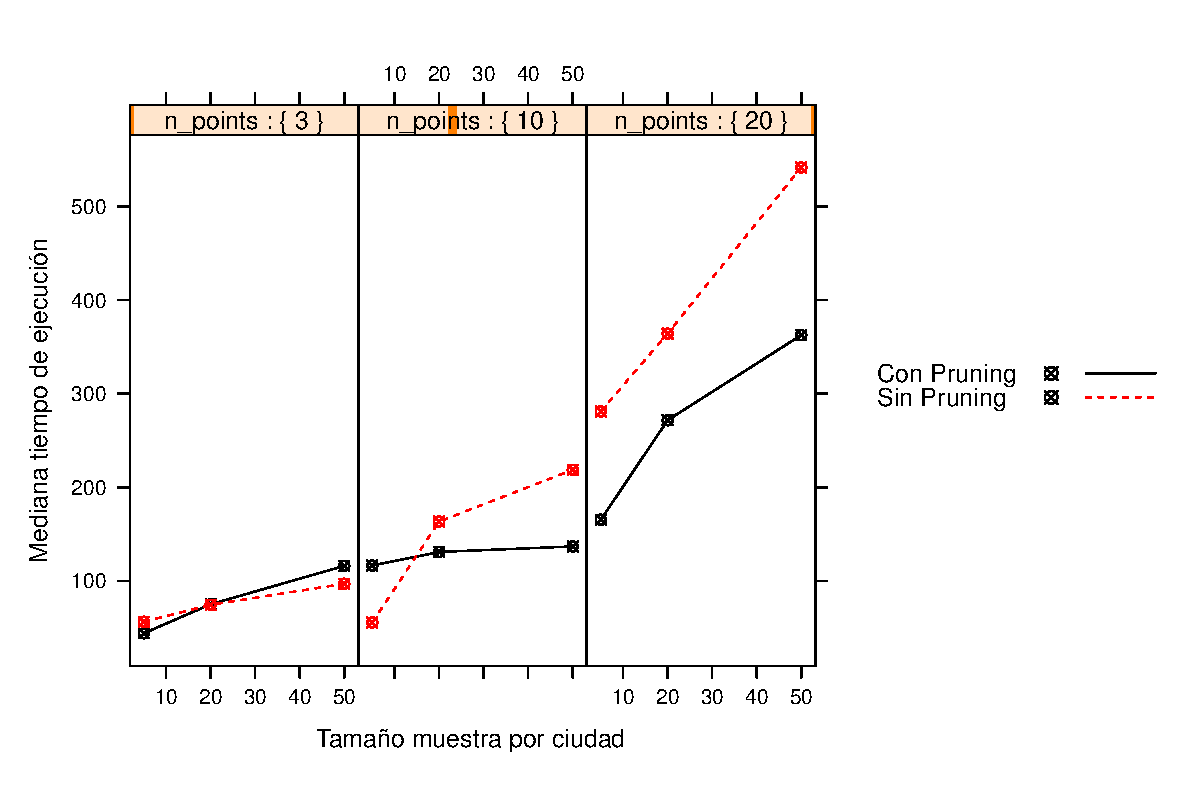
\includegraphics[scale=0.6]{time_mix_ZOIP.eps}	
		\caption{Mediana del tiempo de ejecuci\'{o}n del modelo de regresi\'{o}n ZOIP mixto, bajo la funci\'{o}n de \code{RMM.ZOIP} del paquete \pkg{ZOIP} de \proglang{R}.}
		\label{time_mix_ZOIP}
	\end{center}
\end{figure}

En la figura \ref{time_mix_ZOIP} se muestra la mediana del tiempo de ejecuci\'{o}n de variar, el tama\~{n}o de muestra $n_i$, el n\'{u}mero de puntos de la cuadratura $Q$ y si se utiliza \textit{pruning} o no, sobre el tiempo de ejecuci\'{o}n para el ajuste del modelo de regresi\'{o}n ZOIP mixto, utilizando la funci\'{o}n \code{RMM.ZOIP} del paquete \pkg{ZOIP}, en dicha figura se nota como a medida que se va aumentando el n\'{u}mero de puntos de la cuadratura y el tama\~{n}o de muestra la diferencia de utilizar la metodolog\'{\i}a \textit{pruning} se hace m\'{a}s favorable ya que se nota una reducci\'{o}n significativa en el tiempo de ejecuci\'{o}n del modelo. Por todo el an\'{a}lisis previo hecho con la estimaci\'{o}n de todos los par\'{a}metros de regresi\'{o}n, en el cual se notaba que por lo general sin importar cualquier combinaci\'{o}n entre tama\~{n}o de muestra y el n\'{u}mero de puntos de la cuadratura, la utilizaci\'{o}n de la metodolog\'{\i}a \textit{pruning} no afecta la estimaci\'{o}n de los par\'{a}metros de una manera significa y viendo la figura \ref{time_mix_ZOIP} se ve que es m\'{a}s conveniente utilizar la metodolog\'{\i}a \textit{pruning}, porque esta genera un tiempo de ejecuci\'{o}n m\'{a}s r\'{a}pido para ajustar el modelo y no afecta de manera significativa la estimaci\'{o}n de los efectos fijos ni de los aleatorios del modelo de regresi\'{o}n ZOIP mixto. Adem\'{a}s se puede concluir que el hecho de aumentar el n\'{u}mero de puntos de la cuadratura solo beneficia a la estimaci\'{o}n de los efectos aleatorios mas no de los efectos fijos, en general lo m\'{a}s recomendable para mejorar las estimaciones de todos los par\'{a}metros es aumentar el tama\~{n}o muestra dentro de cada grupo.


%%%%%%%%%%%%%%%%%%%%%%%%%%%%%%%%%%%%%%%%%%%%%%%%%%%%%%%%%%%%%%%%%%%%%%%%%%%%%%%%%%%%%%%%%%%%%%%%%%%%%%%%%%%%%%%%%%%%%%%%%%%%%%%%%%%%%%%%%%%%%%%%%%%%%%%%%%%%%%%%%%

\section{Conclusi\'{o}n}

El modelo de regresi\'{o}n ZOIP con efectos mixtos permite hacer ajustes a un modelo de regresi\'{o}n mixto, donde la variable respuesta est\'{a} dada por datos proporcionales inflados con ceros y/o unos, es decir, bajo una distribuci\'{o}n ZOIP, se considera un modelo de regresi\'{o}n mixto porque adem\'{a}s de considerar efectos fijos sobre cada uno de los par\'{a}metros de la distribuci\'{o}n ZOIP, permite incluir efectos aleatorios, tales como interceptos aleatorios sobre los par\'{a}metros de la media y la dispersi\'{o}n, la estimaci\'{o}n de estos par\'{a}metros se realiza bajo m\'{a}xima verosimilitud y bajo la aproximaci\'{o}n de la cuadratura de Gauss-Hermite adaptativa multidimensional, dicha estimaci\'{o}n puede ser realizada en el paquete \pkg{ZOIP} de \proglang{R}, de una forma muy agradable para el usuario, en el paquete es posible realizar diferentes tipos de regresi\'{o}n ZOIP mixto, bajo diferentes distribuciones y parametrizaciones, adem\'{a}s de obtener resultados del modelo mediante funciones de metodolog\'{\i}a S3 de \proglang{R}.\\

El modelo de regresi\'{o}n ZOIP mixto a manera de resultados, presenta una excelente convergencia de sus par\'{a}metros bajo los estudios de simulaci\'{o}n realizados, adem\'{a}s nos permite concluir que la mejor metodolog\'{\i}a para obtener un buen tiempo de ejecuci\'{o}n y de convergencia de los par\'{a}metros del modelo de regresi\'{o}n ZOIP mixto, es cuando se utiliza un numero prudente de puntos de la cuadratura, es decir, entre cinco y quince puntos, utilizando la metodolog\'{\i}a \textit{pruning} y obteniendo un buen tama\~{n}o de observaciones por cada grupo de la variable de agrupaci\'{o}n del modelo mixto, este tama\~{n}o de muestra es el que mejor efecto obtiene sobre la mejora circunstancial de la convergencia de los par\'{a}metros regresores del modelo de regresi\'{o}n ZOIP mixto. Durante el estudio de simulaci\'{o}n tambi\'{e}n se observ\'{o} que el efecto de aumentar el n\'{u}mero de puntos de la cuadratura, afecta de manera positiva a la convergencia de los par\'{a}metros asociados a los interceptos aleatorios.
